\documentclass[10pt, letterpaper]{article}

% Inhaltsverzeichnis für Pakettypen (nur für Übersicht im Header, wird nicht im Dokument angezeigt)
% 1. Seitenlayout und Ränder
% 2. Sprache und Zeichensatz
% 3. Mathematik und Theorem-Umgebungen
% 4. Eigene Makros
% 5. Diagramme und Grafiken
% 6. Tabellen und Aufzählungen
% 7. Inhaltsverzeichnis
% 8. Abschnittsüberschriften
% 9. Abstrakt-Umgebung
% 10. Todos/Notizen
% 11. Rahmen/Box-Umgebungen
% 12. Python-Integration
% 13. Literaturverwaltung
% 14. Hyperlinks
% 15. Absatzeinstellungen
% 16. Umgebungen
% 17. Titel und Autor

% --- 0. Allgemeine Pakete ---
\usepackage{booktabs}
\usepackage{makecell}
\usepackage{slashed}

% --- 1. Seitenlayout und Ränder ---
\usepackage[margin=3cm]{geometry}

% --- 2. Sprache und Zeichensatz ---
\usepackage[english]{babel}
\usepackage[T1]{fontenc}
\usepackage[utf8]{inputenc}

% --- 3. Mathematik und Theorem-Umgebungen ---
\usepackage{amsmath, amssymb, amsthm}
\usepackage{mathrsfs}
\DeclareMathOperator{\WF}{WF}

% --- 4. Eigene Makros ---
\usepackage{xcolor}
\newcommand{\SKP}{\langle\cdot,\cdot\rangle}
\newcommand{\R}{\mathbb{R}}
\newcommand{\N}{\mathbb{N}}
\newcommand{\Q}{\mathbb{Q}}
\newcommand{\Z}{\mathbb{Z}}
\newcommand{\C}{\mathbb{C}}
\newcommand{\entwurf}[1]{\textcolor{red}{#1}}

% --- 5. Diagramme und Grafiken ---
\usepackage{graphicx}
\graphicspath{{../../Images/}}
\usepackage[export]{adjustbox}
\usepackage{tikz}
\usetikzlibrary{decorations.pathreplacing, arrows.meta, positioning}
\usepackage{tikz-cd}

% --- 6. Tabellen und Aufzählungen ---
\usepackage{enumitem}
\setlist[itemize]{left=0.5cm}

\newenvironment{romanenum}[1][]
  {%
    \ifx&#1&
    \else
      \textbf{#1}\quad
    \fi
    \begin{enumerate}[label=\roman*)]
  }
  {%
    \end{enumerate}%
  }

% --- 7. Inhaltsverzeichnis ---
\usepackage{tocloft}
\renewcommand{\cftsecfont}{\footnotesize}
\renewcommand{\cftsubsecfont}{\footnotesize}
\renewcommand{\cftsubsubsecfont}{\footnotesize}
\renewcommand{\cftsecpagefont}{\footnotesize}
\renewcommand{\cftsubsecpagefont}{\footnotesize}
\renewcommand{\cftsubsubsecpagefont}{\footnotesize}
\usepackage{etoc}

% --- 8. Abschnittsüberschriften ---
\usepackage{titlesec}
\titleformat{\section}{\normalfont\large\bfseries}{\thesection}{1em}{}
\titleformat{\subsection}{\normalfont\normalsize\bfseries}{\thesubsection}{0.5em}{}
\titleformat{\subsubsection}{\normalfont\normalsize\bfseries}{\thesubsubsection}{0.5em}{}
\setcounter{secnumdepth}{4}

% --- 9. Abstrakt-Umgebung ---
\usepackage{changepage}
\renewenvironment{abstract}
  {
    \begin{adjustwidth}{1.5cm}{1.5cm}
    \small
    \textsc{Abstract. –}%
  }
  {
    \end{adjustwidth}
  }

% --- 10. Todos/Notizen ---
\usepackage{todonotes}
% Hellblau definieren
\definecolor{hellblau}{rgb}{0.3,0.6,1}

% Eigene Umgebung »notiz«
\newenvironment{note}{\par\begingroup\color{hellblau}\itshape}{\par\endgroup}

% --- 11. Rahmen/Box-Umgebungen ---
\usepackage{mdframed}
\usepackage{tcolorbox}
\colorlet{shadecolor}{gray!25}

\newenvironment{customTheorem}
  {\vspace{10pt}%
   \begin{mdframed}[
     backgroundcolor=gray!20,
     linewidth=0pt,
     innertopmargin=10pt,
     innerbottommargin=10pt,
     skipabove=\dimexpr\topsep+\ht\strutbox\relax,
     skipbelow=\topsep,
   ]}
  {\end{mdframed}
   \vspace{10pt}%
  }

% --- 12. Python-Integration ---
% (Deaktiviert in dieser Version, aktiviere bei Bedarf)
% \usepackage{pythontex}
% \usepackage[makestderr]{pythontex}

% --- 13. Literaturverwaltung ---
\usepackage{csquotes}
\usepackage[backend=biber, style=alphabetic, citestyle=alphabetic]{biblatex}
\addbibresource{bibliography.bib}

% --- 14. Hyperlinks ---
\usepackage{hyperref}
\hypersetup{
  colorlinks   = true,
  urlcolor     = blue,
  linkcolor    = blue,
  citecolor    = blue,
  frenchlinks  = true
}

% --- 15. Absatzeinstellungen ---
\usepackage[parfill]{parskip}
\sloppy

% --- 16. Umgebungen ---
\usepackage{thmtools}

\newcommand{\CustomHeading}[3]{%
  \par\medskip\noindent%
  \textbf{#1 #2} \textnormal{(#3)}.\enskip%
}

\newenvironment{DEF}[2]{\CustomHeading{Definition}{#1}{#2}}{}
\newenvironment{PROP}[2]{\CustomHeading{Proposition}{#1}{#2}}{}
\newenvironment{THEO}[2]{\CustomHeading{Theorem}{#1}{#2}}{}
\newenvironment{LEM}[2]{\CustomHeading{Lemma}{#1}{#2}}{}
\newenvironment{KORO}[2]{\CustomHeading{Corollar}{#1}{#2}}{}
\newenvironment{REM}[2]{\CustomHeading{Remark}{#1}{#2}}{}
\newenvironment{EXA}[2]{\CustomHeading{Example}{#1}{#2}}{}
\newenvironment{STUD}[2]{\CustomHeading{Study}{#1}{#2}}{}
\newenvironment{CONC}[2]{\CustomHeading{Concept}{#1}{#2}}{}
\newenvironment{OTH}[2]{\CustomHeading{Other}{#1}{#2}}{}
\newenvironment{EXE}[2]{\CustomHeading{Exercise}{#1}{#2}}{}
\newenvironment{MOT}[2]{\CustomHeading{Motivation}{#1}{#2}}{}
\newenvironment{PROOF}[2]{\CustomHeading{Proof}{#1}{#2}}{}



% --- Unit Umgebung ---
\usepackage{mdframed}
\newmdenv[
  linewidth=1pt,
  topline=false,
  bottomline=false,
  rightline=false,
  leftmargin=0cm,
  rightmargin=0cm,
  skipabove=10pt,
  skipbelow=10pt,
  innertopmargin=0.5\baselineskip,
  innerbottommargin=0.5\baselineskip,
  backgroundcolor=gray!10,
  linecolor=gray
]{unitbox}

\newenvironment{unit}[1]
  {\begin{unitbox}\textbf{Unit #1}\par\smallskip}
  {\end{unitbox}}


% --- 17. Titel und Autor ---
\title{Mein Titel}
\author{Tim Jaschik}
\date{\today}

\begin{document}

\maketitle
\rule{\textwidth}{0.5pt}
\begin{abstract}
Kurze Beschreibung …
\end{abstract}
\rule{\textwidth}{0.5pt}
\vspace{0.5cm}

\tableofcontents

\pagebreak

\section{Grundlagen}

\subsection{Formalismen}

\begin{CONC}{CM-K25c-09-01}{Alembert Prinzip}
Gegeben sei ein System aus $N$ Massenpunkten, auf die Zwangkräfte 
$\vec Z_i$ wirken.  
Nach dem d’Alembert-Prinzip verschwindet die Summe der von den 
$\vec Z_i$ verrichteten \emph{virtuellen} Arbeit:
\[
  \boxed{\;
    \delta W \;=\;\sum_{i=1}^{N}\vec Z_i\!\cdot\!\delta\vec r_i \;=\;0
  \;}
\]

\textbf{Virtuelle Verrückung $\delta\vec r_i$}
\begin{itemize}
  \item infinitesimal klein,
  \item verträglich mit allen Zwangsbedingungen,
  \item \emph{zeitlos} ($\delta t=0$): während $\delta\vec r_i$ werden 
        die ZB nicht verletzt.
\end{itemize}
\end{CONC}

\begin{REM}{CM-K25c-09-02}{Alembert Prinzip h d rheonomische ZB}
Bei zeitabhängigen (rheonomischen) ZB gilt zwar immer 
$\vec Z_i\!\cdot\!\delta\vec r_i=0$,  
doch die \emph{reale} Arbeit $\vec Z_i\!\cdot\!d\vec r_i$ kann ungleich 
Null sein.
\end{REM}

\begin{CONC}{CM-K25c-09-04}{Herleitung der d’Alembert-Gleichungen}
Aus den Newton’schen Gleichungen
\[
  m_i\ddot{\vec r}_i = \vec F_i + \vec Z_i,
  \qquad i=1,\dots,N,
\]
folgt nach Skalar­produkt mit $\delta\vec r_i$ und Summation:
\[
  \sum_{i=1}^{N}\bigl(m_i\ddot{\vec r}_i - \vec F_i\bigr)\!\cdot\!\delta\vec r_i
  = \sum_{i=1}^{N}\vec Z_i\!\cdot\!\delta\vec r_i = 0.
\]
Dies ist die \emph{d’Alembert-Gleichung}
\[
  \boxed{\;
    \sum_{i=1}^{N}\bigl(m_i\ddot{\vec r}_i - \vec F_i\bigr)
    \!\cdot\!\delta\vec r_i = 0
  \;}
\]
\end{CONC}

\begin{CONC}{CM-K25c-09-05}{Übergang zur Bewegungsgleichung für generelle Koordinaten}
Seien $k$ holonome ZB vorhanden ($n=M-k$ unabhängig).  
Schreibe
\[
  \vec r_i = \vec r_i(q_1,\dots,q_n,t)
  \quad\Longrightarrow\quad
  \delta\vec r_i = \sum_{j=1}^{n}
                   \frac{\partial\vec r_i}{\partial q_j}\,\delta q_j .
\]
Einsetzen in die d’Alembert-Gleichung liefert
\[
  \sum_{j=1}^{n}\!
  \Biggl[
    \sum_{i=1}^{N}
      \bigl(m_i\ddot{\vec r}_i - \vec F_i\bigr)
      \!\cdot\!
      \frac{\partial\vec r_i}{\partial q_j}
  \Biggr]\!
  \delta q_j = 0 .
\]
Da die $\delta q_j$ unabhängig sind, muss jede Klammer verschwinden:
\[
  \boxed{\;
    \sum_{i=1}^{N}\!
      \bigl(m_i\ddot{\vec r}_i - \vec F_i\bigr)
      \!\cdot\!
      \frac{\partial\vec r_i}{\partial q_j}
    = 0,
    \quad j=1,\dots,n.
  \;}
\]
Dies sind $n$ Bewegungsgleichungen für die unabhängigen Koordinaten 
$q_j$ – ohne explizite Zwangkräfte. Sie bilden den Ausgangspunkt der Lagrange’schen Formulierung.
\end{CONC}

\begin{CONC}{CM-K25c-09-07}{Rezept: Bewegungsgleichungen aus der d’Alembert-Gleichung}
\textbf{Vorgehen}\\[-4pt]
\begin{enumerate}
  \item Schreibe die d’Alembert-Gleichung in kartesischen Koordinaten
        \[
          \sum_{i=1}^{N}
            \bigl(m_i\ddot{\vec r}_i-\vec F_i\bigr)\!\cdot\!\delta\vec r_i = 0 .
        \]
  \item Drücke alle kartesischen Koordinaten $\vec r_i$ mittels der
        unabhängigen generalisierten Koordinaten
        $q_1,\dots,q_n$ (und ggf.\ $t$) aus; ersetze entsprechend
        $\delta\vec r_i$.
  \item Setze die (linear unabhängigen) Koeffizienten der Variationen
        $\delta q_j$ gleich Null.  
        Dies liefert $n$ Bewegungsgleichungen für
        $q_1(t),\dots,q_n(t)$ ohne explizite Zwangkräfte.
\end{enumerate}
\end{CONC}

\begin{CONC}{CM-K25c-09-08}{Gleichgewichtsprinzip}
Im statischen Gleichgewicht gilt $\ddot{\vec r}_i=0$. Die d’Alembert-Gleichung reduziert sich auf
\[
  \sum_{i=1}^{N}\vec F_i\!\cdot\!\delta\vec r_i = 0 .
\]
Damit verschwindet die virtuelle Arbeit aller äußeren Kräfte
im Gleichgewicht.
\end{CONC}

\begin{CONC}{CM-K25c-09-09}{Bestimmung von Zwangkräften über ein virtuelles Zusatz­system}
Soll eine bestimmte Zwangkraft $\vec Z^{\ast}$ berechnet werden, behandelt man sie gedanklich als
\emph{eingeprägte} (äußere) Kraft; die zugehörige ZB ist damit vorübergehend aufgehoben. Das System erhält dadurch einen zusätzlichen Freiheitsgrad. Die d’Alembert-Gleichung liefert nun eine weitere Bedingung, aus der $\vec Z^{\ast}$ (als unbekannte eingeprägte Kraft) algebraisch bestimmt werden kann. Auf diese Weise lässt sich die gesuchte Zwangkraft ermitteln, ohne alle anderen Reaktionskräfte explizit zu kennen.
\end{CONC}

\begin{CONC}{CM-K25c-09-11}{Zwangkräfte als Normalenkräfte und Ursprung des d’Alembert-Prinzips}
\textbf{Erfahrungstatsache}\\
Für einen Massenpunkt, dessen Bewegung durch eine \emph{holonome}
Zwangsbedingung
\[
  f\!\bigl(\vec r,t\bigr)=0
\]
eingeschränkt ist, gilt empirisch
\[
  \boxed{\;
    \vec Z = m\ddot{\vec r}-\vec F
    = \lambda(\vec r,\dot{\vec r},t)\,
      \nabla_{\!\vec r} f(\vec r,t)
  \;}
\]
mit einem skalar-wertigen Lagrange-Multiplikator $\lambda$.  
Da $\nabla_{\!\vec r}f$ senkrecht auf der Fläche $f=\text{const}$
steht, wirkt die Zwangkraft \emph{normal} auf die Bahnfläche.

\textbf{Folgerung}\\
Virtuelle Verrückungen $\delta\vec r$ sind tangential zur
Bahnfläche und erfüllen
\[
  \nabla_{\!\vec r} f\!\cdot\!\delta\vec r = 0
  \;\;\Longrightarrow\;\;
  \vec Z\!\cdot\!\delta\vec r
  = \lambda\,\nabla_{\!\vec r}f\!\cdot\!\delta\vec r = 0 .
\]
Damit folgt unmittelbar das d’Alembert-Prinzip
$\sum\vec Z_i\!\cdot\!\delta\vec r_i = 0$.
\end{CONC}

\begin{CONC}{CM-K25c-09-13}{Verallgemeinerung auf $N$ Teilchen und $k$ Zwangsbedingungen}
\textbf{a) Holonome Zwangsbedingungen}\\
Sind $k$ unabhängige, holonome Bedingungen
\[
  f_j\!\bigl(\vec r_1,\dots,\vec r_N,t\bigr)=0,
  \qquad j=1,\dots,k
\]
gegeben, so hat jede Zwangskraft die Gestalt
\[
  \boxed{\,%
    \vec Z_i =
    \sum_{j=1}^{k}
      \lambda_j(\vec r_1,\dots,\vec r_N,
                \dot{\vec r}_1,\dots,\dot{\vec r}_N,t)\,
      \nabla_{\!\vec r_i} f_j(\vec r_1,\dots,\vec r_N,t)
    \,}, \qquad i=1,\dots,N.
\]
Setzt man
\[
  \vec a_{ji}(\vec r_1,\dots,\vec r_N,t)
  :=\nabla_{\!\vec r_i} f_j(\vec r_1,\dots,\vec r_N,t),
\]
so lautet dieselbe Beziehung kurz
\[
  \vec Z_i = \sum_{j=1}^{k}\lambda_j\,\vec a_{ji}.
\]
Für Punktmassen in allgemeinen Koordinaten
\(
  q_1,\dots,q_M
\)
erscheint $\vec a_{ji}$ als
\(
  a_{ji}=\partial h_j/\partial q_i
\)
(vgl.\ Kap.~2.1\,c).

\textbf{b) Differential-Zwangsbedingungen}\\
Liegen die $k$ Bedingungen nur in Pfaffscher Form vor
\[
  \sum_{i=1}^{N}\vec a_{ji}\!\cdot d\vec r_i + a_{jt}\,dt = 0,
  \qquad j=1,\dots,k,
\]
so gilt analog
\[
  \boxed{\,%
    \vec Z_i = \sum_{j=1}^{k}\lambda_j\,\vec a_{ji},
    \qquad i=1,\dots,N.%
  \,}
\]
\end{CONC}

\begin{CONC}{CM-K25c-09-14}{Verallgemeinerung auf $N$ Teilchen Herleitung der AP}
\textbf{Virtuelle Verrückungen}\\
Für eine holonome Bedingung folgt
\[
  0 = \delta f_j
    = \sum_{i=1}^{N}\nabla_{\!\vec r_i}f_j\!\cdot\!\delta\vec r_i
    = \sum_{i=1}^{N}\vec a_{ji}\!\cdot\!\delta\vec r_i,
\]
und bei Pfaffschen ZB gilt wegen $\delta t=0$ dasselbe Resultat.

\textbf{Virtuelle Arbeit der Zwangkräfte}\\
\[
  \sum_{i=1}^{N}\vec Z_i\!\cdot\!\delta\vec r_i
  = \sum_{i=1}^{N}
      \Bigl(\sum_{j=1}^{k}\lambda_j\,\vec a_{ji}\Bigr)
      \!\cdot\!\delta\vec r_i
  = \sum_{j=1}^{k}\lambda_j
      \Bigl(\sum_{i=1}^{N}\vec a_{ji}\!\cdot\!\delta\vec r_i\Bigr)
  = 0.
\]
Damit ergibt sich unmittelbar das \emph{d’Alembert-Prinzip}
\[
  \boxed{\;
    \sum_{i=1}^{N}\vec Z_i\!\cdot\!\delta\vec r_i = 0
  \;}
\]
als Konsequenz der Tatsache, dass Zwangkräfte stets normal auf
den vom System einzuhaltenden Zwangsflächen bzw.\ -bahnen stehen.
\end{CONC}

\begin{CONC}{CM-K25c-09-15}{Übersicht zentraler Sätze des Lagrange Formalismus}
\begin{enumerate}
  \item \textbf{d’Alembert-Prinzip}  
        \[
          \boxed{\;
            \sum_{i=1}^{N} \vec Z_i \!\cdot\! \delta\vec r_i = 0
          \;}
        \]
        Die gesamte virtuelle Arbeit der Zwangkräfte verschwindet.

  \item \textbf{d’Alembert-Gleichung}  
        \[
          \boxed{\;
            \sum_{i=1}^{N}
              \bigl(m_i\ddot{\vec r}_i - \vec F_i\bigr)
              \!\cdot\! \delta\vec r_i = 0
          \;}
        \]
        Durch Einbeziehen der Trägheitskräfte wird die Wirkung der
        Zwangkräfte eliminiert.

  \item \textbf{Bewegungsgleichungen in unabhängigen
        Koordinaten\,$q_1,\dots,q_n$}  
        Bei $k$ holonomen Bedingungen ($n=M-k$):
        \[
          \boxed{\;
            \sum_{i=1}^{N}
              \bigl(m_i\ddot{\vec r}_i - \vec F_i\bigr)
              \!\cdot\!
              \frac{\partial\vec r_i}{\partial q_j}
            = 0,
            \quad j=1,\dots,n
          \;}
        \]
        Dies sind $n$ Differentialgleichungen ohne explizite
        Zwangkräfte.

  \item \textbf{Gleichgewichtsprinzip}  
        \[
          \boxed{\;
            \sum_{i=1}^{N} \vec F_i \!\cdot\! \delta\vec r_i = 0
          \;}
        \]
        Im statischen Gleichgewicht (\,${\ddot{\vec r}}_i=0$\,) leistet
        die Gesamtheit der eingeprägten Kräfte keine virtuelle Arbeit.
\end{enumerate}
\end{CONC}

\begin{CONC}{CM-K25c-10-01}{Herleitung der Lagrange-Gleichungen 2. Art aus der d’Alembert-Gleichung}
\textbf{1.\ Ausgangspunkt: d’Alembert-Gleichung}

\[
  \sum_{i=1}^{N}\bigl(m_i\ddot{\vec r}_i-\vec F_i\bigr)\!\cdot\!\delta\vec r_i=0.
\]

\textbf{2.\ Verallgemeinerte Koordinaten}

Wähle $n$ (später unabhängige) Koordinaten $q_1,\dots,q_n$  
und setze
\[
  \vec r_i=\vec r_i(q_1,\dots,q_n,t),
  \qquad
  \delta\vec r_i=\sum_{j=1}^{n}
                  \frac{\partial\vec r_i}{\partial q_j}\,\delta q_j.
\]

\textbf{3.\ Generalisierte Kräfte}

\[
  \sum_{i=1}^{N}\vec F_i\!\cdot\!\delta\vec r_i
  =\sum_{j=1}^{n}
     \underbrace{\Bigl(
       \sum_{i=1}^{N}\vec F_i\!\cdot\!
       \frac{\partial\vec r_i}{\partial q_j}
     \Bigr)}_{=:\,Q_j}
     \delta q_j.
\]

\textbf{4.\ Transformation des Trägheitsterms}

\[
\begin{aligned}
  \sum_{i=1}^{N}m_i\ddot{\vec r}_i\!\cdot\!\delta\vec r_i
  &=\sum_{j=1}^{n}\!
     \Bigl[
       \sum_{i=1}^{N}
         m_i\ddot{\vec r}_i\!\cdot\!
         \frac{\partial\vec r_i}{\partial q_j}
     \Bigr]\delta q_j\\[2pt]
  &=\sum_{j=1}^{n}\!
     \Bigl[
       \frac{\mathrm d}{\mathrm dt}
         \Bigl(
           \sum_{i=1}^{N}
             m_i\dot{\vec r}_i\!\cdot\!
             \frac{\partial\vec r_i}{\partial q_j}
         \Bigr)
       -
       \sum_{i=1}^{N}
         m_i\dot{\vec r}_i\!\cdot\!
         \frac{\mathrm d}{\mathrm dt}
           \frac{\partial\vec r_i}{\partial q_j}
     \Bigr]\delta q_j .
\end{aligned}
\]

Da
\(
  \dfrac{\mathrm d}{\mathrm dt}
  \dfrac{\partial\vec r_i}{\partial q_j}
  =
  \dfrac{\partial\dot{\vec r}_i}{\partial q_j},
\)
ergibt sich mit
\(
  T=\sum_{i=1}^{N}\tfrac12m_i\dot{\vec r}_i^{\,2}
\)

\[
  \sum_{i=1}^{N}m_i\ddot{\vec r}_i\!\cdot\!\delta\vec r_i
  =
  \sum_{j=1}^{n}
    \Bigl[
      \frac{\mathrm d}{\mathrm dt}
        \Bigl(\frac{\partial T}{\partial\dot q_j}\Bigr)
      -
      \frac{\partial T}{\partial q_j}
    \Bigr]\delta q_j .
\]

\textbf{5.\ d’Alembert–Lagrange-Gleichung}

Einsetzen in die d’Alembert-Gleichung liefert

\[
  \sum_{j=1}^{n}
    \Bigl[
      \frac{\mathrm d}{\mathrm dt}\frac{\partial T}{\partial\dot q_j}
      -
      \frac{\partial T}{\partial q_j}
      -
      Q_j
    \Bigr]\delta q_j=0.
\]

Bei $k$ holonomen ZB sind $n=3N-k$ Koordinaten unabhängig, also

\[
  \boxed{\;
    \frac{\mathrm d}{\mathrm dt}\frac{\partial T}{\partial\dot q_j}
    -
    \frac{\partial T}{\partial q_j}
    =Q_j,
    \qquad j=1,\dots,n .\;}
\]

\textbf{6.\ Einführung eines (generalisierten) Potentials}

\begin{itemize}
\item \textbf{Konservative Kräfte}  
      $\vec F_i=-\nabla_{\vec r_i}V(\vec r_1,\dots,\vec r_N,t)$  
      $\Longrightarrow\;Q_j=-\dfrac{\partial V}{\partial q_j}$.
\item \textbf{Geschwindigkeitsabhängige Kräfte}  
      Existiert ein \emph{generalisiertes Potential}
      $V(q,\dot q,t)$ mit
      \[
        Q_j=-\frac{\partial V}{\partial q_j}
            +\frac{\mathrm d}{\mathrm dt}
             \frac{\partial V}{\partial\dot q_j},
      \]
      dann bleibt die Struktur erhalten.
\end{itemize}

\textbf{7.\ Lagrange-Funktion und Gleichungen 2.\ Art}

Definiere
\[
  L(q,\dot q,t)=T(q,\dot q,t)-V(q,\dot q,t).
\]
Dann wird die letzte Gleichung zu

\[
  \boxed{\;
    \frac{\mathrm d}{\mathrm dt}\frac{\partial L}{\partial\dot q_j}
    -
    \frac{\partial L}{\partial q_j}=0,
    \qquad j=1,\dots,n
  \;}
\]

– den \emph{Lagrange-Gleichungen 2.\ Art}.  
Sie gelten genau dann, wenn
\begin{itemize}
  \item die Zwangbedingungen holonom sind und
  \item alle eingeprägten Kräfte aus einem (möglicherweise
        geschwindigkeitsabhängigen) Potential stammen.
\end{itemize}
\end{CONC}

\begin{CONC}{CM-K25c-10-04}{Forminvarianz der Lagrangegleichungen unter Punkttransformation}
%--------------------------------------------------------------------
\textbf{Forminvarianz der Lagrange-Gleichungen}
%--------------------------------------------------------------------

Gegeben sei eine Lagrange-Funktion
\[
  L(q_1,\dots,q_n,\dot q_1,\dots,\dot q_n,t),
  \qquad
  n = 3N-k ,
\]
für die bereits gilt
\[
  \boxed{%
    \frac{\mathrm d}{\mathrm dt}\frac{\partial L}{\partial\dot q_j}
    -\frac{\partial L}{\partial q_j}=0,
    \quad j=1,\dots,n }.
\]

\textbf{Punkttransformation}\\
Wir führen eine reguläre (d.\,h. invertierbare) Punkttransformation ein  
\[
  q'_j = q'_j(q_1,\dots,q_n,t),
  \qquad
  (J:=\det{\partial q'_j/\partial q_i}\neq0),
\]
mit der Inversen
\( q_i = q_i(q'_1,\dots,q'_n,t) \).
Die neuen Geschwindigkeiten sind
\[
  \dot q_i(q',\dot q',t)
  =\sum_{k=1}^{n}\frac{\partial q_i}{\partial q'_k}\,\dot q'_k
   +\frac{\partial q_i}{\partial t}.
\]

\textbf{Transformation der Lagrange-Funktion}\\
\[
  \boxed{%
    L'(q',\dot q',t)
    =L\!\bigl(q(q',t),\dot q(q',\dot q',t),t\bigr)}.
\]
$L'$ ist also ein \emph{Skalar}: sein numerischer Wert bleibt erhalten,
nur die Darstellung in den Koordinaten ändert sich.

%--------------------------------------------------------------------
\textbf{Ableitungen von $L'$}
%--------------------------------------------------------------------
\[
  \frac{\partial L'}{\partial q'_j}
  =\sum_{i=1}^{n}\Bigl(
      \frac{\partial L}{\partial q_i}\,
      \frac{\partial q_i}{\partial q'_j}
     +\frac{\partial L}{\partial\dot q_i}\,
      \frac{\partial\dot q_i}{\partial q'_j}\Bigr),\qquad
  \frac{\partial L'}{\partial\dot q'_j}
  =\sum_{i=1}^{n}
      \frac{\partial L}{\partial\dot q_i}\,
      \frac{\partial q_i}{\partial q'_j}.
\]
Dabei wurden die elementaren Beziehungen
\[
  \boxed{%
    \frac{\partial\dot q_i}{\partial\dot q'_j}=
    \frac{\partial q_i}{\partial q'_j}},
  \qquad
  \boxed{%
    \frac{\mathrm d}{\mathrm dt}
    \Bigl(\frac{\partial q_i}{\partial q'_j}\Bigr)=
    \frac{\partial\dot q_i}{\partial q'_j}}
\]
genutzt (direkte Ableitung und Vertauschung der partiellen Differentiationen).

%--------------------------------------------------------------------
\textbf{Lagrange-Gleichungen in den neuen Koordinaten}
%--------------------------------------------------------------------
\[
\begin{aligned}
  \frac{\mathrm d}{\mathrm dt}
    \Bigl(\frac{\partial L'}{\partial\dot q'_j}\Bigr)
  -\frac{\partial L'}{\partial q'_j}
  &=
  \sum_{i=1}^{n}
    \Bigl[\,
      \frac{\mathrm d}{\mathrm dt}
        \Bigl(\frac{\partial L}{\partial\dot q_i}\Bigr)
      -\frac{\partial L}{\partial q_i}\Bigr]
    \frac{\partial q_i}{\partial q'_j}\;=\;0 .
\end{aligned}
\]
Der letzte Schritt folgt, weil der Klammerausdruck für jedes
$i$ aufgrund der ursprünglichen Lagrange-Gleichungen verschwindet.
Damit ist bewiesen:

\[
  \boxed{%
    \frac{\mathrm d}{\mathrm dt}
      \frac{\partial L'}{\partial\dot q'_j}
    -\frac{\partial L'}{\partial q'_j}=0,
    \quad j=1,\dots,n }.
\]

%--------------------------------------------------------------------
\textbf{Ergebnis}
%--------------------------------------------------------------------
Die Lagrange-Gleichungen sind \emph{forminvariant} unter beliebigen
regulären Punkttransformationen
\( q\mapsto q'(q,t) \).
Insbesondere behalten sie ihre Gestalt auch in beschleunigten
(Bezugs-) Koordinatensystemen.
\end{CONC}

\begin{CONC}{CM-K25c-10-06}{Symmetrien Invarianzen Erhaltungsgrößen}
\begin{enumerate}

%--------------------------------------------------------------
\item \textbf{Symmetrie}  
Ein mechanisches System ist \emph{symmetrisch} gegenüber einer
Operation, wenn sich sein beobachtbarer Zustand nach Ausführung der
Operation nicht ändert.

\textit{Beispiel:} Eine perfekte Kugel bleibt unter beliebiger
Drehung um ihren Mittelpunkt unverändert.

%--------------------------------------------------------------
\item \textbf{Invarianz der Lagrange-Funktion}  
Sei die Operation durch eine Punkt­transformation
$\,q_i\mapsto q'_i(q,t)$ beschrieben.
Unter allgemeinen Punkt­transformationen verhält sich die
Lagrange-Funktion wie ein Skalar:
\[
  L'(q',\dot q',t)
  \;=\;
  L\!\bigl(q(q',t),\;\dot q(q',\dot q',t),\;t\bigr).
\]
\emph{Invarianz} liegt vor, wenn zugleich
\[
  L'(q',\dot q',t)
  =L\!\bigl(q'\!,\dot q',t\bigr),
\]
d.\,h. die funktionale Gestalt bleibt identisch.

\textit{Beispiel (symmetrisch):} Teilchen im rotations­invarianten
Potential  
$L=\tfrac{m}{2}(\dot x^2+\dot y^2+\dot z^2)-V(x^2+y^2,z)$  
ist invariant unter
$(x,y)\mapsto(x\cos\alpha-y\sin\alpha,\;x\sin\alpha+y\cos\alpha)$.

\textit{Beispiel (nicht symmetrisch):}  
Freies Teilchen  
$L=\tfrac{m}{2}\dot x^{2}$
in ein beschleunigtes Bezugs­system  
$x'=x-\!\int_0^t\!V(t')dt'$ überführt:
\[
  L'=\tfrac{m}{2}(\dot x'+V)^{2}\neq L(x'\!,\dot x',t).
\]

%--------------------------------------------------------------
\item \textbf{Erhaltungsgröße}  
Eine Größe
$f(q,\dot q,t)$ heißt \emph{erhalten}, wenn für jede Lösung
$q(t)$ der Lagrange-Gleichungen
\[
  \frac{d}{dt}\,f(q,\dot q,t)=0.
\]

%--------------------------------------------------------------
\item \textbf{Kanonischer (generaliserter) Impuls}  
Zu jeder Koordinate $q_i$:
\[
  p_i=\frac{\partial L}{\partial\dot q_i},
  \qquad
  \dot p_i=\frac{\partial L}{\partial q_i}.
\]

\textit{Beispiel:} Geladenes Teilchen im EM-Feld  
$L=\tfrac{m}{2}\dot{\vec r}^{\,2}-Q(\phi-\dot{\vec r}\!\cdot\!\vec A/c)$  
liefert
\[
  \vec p=m\dot{\vec r}+\frac{Q}{c}\vec A
\]
(konjugierter Impuls $\neq$ kinematischer Impuls).

%--------------------------------------------------------------
\item \textbf{Zyklische Koordinate}  
Eine Koordinate $q_i$, die in $L$ nicht explizit vorkommt
\[
  \frac{\partial L}{\partial q_i}=0,
\]
führt unmittelbar zu einer Erhaltungsgröße:
\[
  \frac{d}{dt}\bigl(\tfrac{\partial L}{\partial\dot q_i}\bigr)=0
  \;\Longrightarrow\;
  p_i=\text{const}.
\]

\textit{Beispiel:} Teilchen auf Kreiskegel  
\[
  L=\frac{m}{2}
     \Bigl((1+\cos^{2}\alpha)\dot s^{2}+s^{2}\dot\varphi^{2}\Bigr)
     -mg s\cos\alpha,
\]
$\varphi$ ist zyklisch $\Rightarrow$
$p_\varphi=m s^{2}\dot\varphi=\text{const}$ (Drehimpuls).

\end{enumerate}

%--------------------------------------------------------------------
\textbf{Nutzung von Erhaltungsgrößen}  
Zyklische Koordinaten und die zugehörigen Erhaltungsgrößen erleichtern
die analytische Lösung (Trennung der Variablen, Reduktion der Ordnung)
und liefern unmittelbare Einsichten in den Bewegungsablauf (Richtung
des Drehimpulses, Energiebilanz etc.).

%--------------------------------------------------------------------
\textbf{Zusammenhang mit dem Noether-Theorem}  
Jede stetige Symmetrie (Invarianz der Lagrange-Funktion) erzeugt eine
Erhaltungsgröße.  
Zyklische Koordinaten sind das einfachste Beispiel: die Verschiebung
$q_i\!\to\!q_i+\text{const}$ ist eine Symmetrie $\Rightarrow$
Erhaltung von $p_i$.
\end{CONC}

\begin{CONC}{CM-K25c-10-07}{Noether-Theorem}
\textbf{Aussage}\\
Eine stetige Symmetrietransformation der Koordinaten
\[
  q_i \;\longrightarrow\; q'_i(q,t;\alpha),
  \qquad
  q'_i(q,t;0)=q_i,
  \qquad
  i=1,\dots,n
\]
führt – sofern die Lagrange-Funktion invariant bleibt –
zu einer Erhaltungsgröße.

%--------------------------------------------------------------

\textbf{Voraussetzungen}
\begin{itemize}
  \item Punkttransformation mit kleinem Parameter $\alpha$
        (invertierbar, differenzierbar).
  \item Invarianz der Lagrange-Funktion
        \[
          L'(q',\dot q',t;\alpha)
          =
          L\bigl(q(q',t;\alpha),\dot q(q',\dot q',t;\alpha),t\bigr)
          =
          L(q',\dot q',t).
        \]
\end{itemize}

%--------------------------------------------------------------
\textbf{Ableitung}
Differentiation nach $\alpha$ bei festen $q',\dot q'$ ergibt
\[
\begin{aligned}
  0
  &=\frac{\partial L'}{\partial\alpha}
    =\sum_{i=1}^{n}
      \Bigl(
        \frac{\partial L}{\partial q_i}\,
        \frac{\partial q_i}{\partial\alpha}
       +\frac{\partial L}{\partial\dot q_i}\,
        \frac{d}{dt}\frac{\partial q_i}{\partial\alpha}
      \Bigr)\\
  &=\frac{d}{dt}
      \Bigl(
        \sum_{i=1}^{n}
          \frac{\partial L}{\partial\dot q_i}\,
          \frac{\partial q_i}{\partial\alpha}
      \Bigr) .
\end{aligned}
\]
Dabei wurden die Lagrange-Gleichungen
$\smash{\tfrac{d}{dt}\bigl(\partial L/\partial\dot q_i\bigr)
       =\partial L/\partial q_i}$ benutzt.

%--------------------------------------------------------------
\textbf{Erhaltungsgröße (Noether-Invariante)}
Für $\alpha=0$ erhält man die konstante Größe
\[
  \boxed{%
    I(q,\dot q,t)
    =\sum_{i=1}^{n}
      p_i\,
      \Bigl.
        \dfrac{\partial q_i(q',t;\alpha)}{\partial\alpha}
      \Bigr|_{\alpha=0}},
  \qquad
  p_i=\dfrac{\partial L}{\partial\dot q_i}.
\]
Da $\dfrac{dI}{dt}=0$ entlang jeder Lösung, ist $I$ eine
\emph{Erhaltungsgröße}.  
Dies fasst den Zusammenhang
\[
  \text{Symmetrie} \;\Longrightarrow\; \text{Invarianz von } L
  \;\Longrightarrow\; \text{Erhaltungsgesetz}
\]
präzise zusammen.
\end{CONC}

\begin{CONC}{CM-K25c-10-08}{Allgemeine Form des Noether-Theoremsn}
\textbf{1. Quasi-Invarianz der Lagrange-Funktion}

Eine stetige, einparametrige Punkttransformation
\[
  q_i \;\longrightarrow\; q'_i(q,t;\alpha),
  \qquad
  q'_i(q,t;0)=q_i,
  \qquad i=1,\dots,n
\]
heiße \emph{Symmetrietransformation}, wenn sie die Lagrange-Funktion nur
um eine totale Zeitableitung ändert
\begin{equation}
  L'(q',\dot q',t;\alpha)
  \;=\;
  L(q',\dot q',t)
  +\frac{\mathrm d}{\mathrm dt}\,F(q',t;\alpha) ,
  \label{eq:quasiinv}
\end{equation}
wobei \(F\) eine beliebige skalare Funktion ist.  
Die Bewegungsgleichungen bleiben dadurch unverändert
(\emph{Eich-Invarianz}).  

\textbf{Lemma (Eich-Invarianz).}  
Für jede Funktion \(F(q,t)\) haben
\[
  L \quad\text{und}\quad 
  \tilde L=L+\frac{\mathrm dF}{\mathrm dt}
\]
identische Euler-Lagrange-Gleichungen.

\emph{Beweis.}
\[
  \frac{\mathrm d}{\mathrm dt}\frac{\partial\tilde L}{\partial\dot q_i}
 -\frac{\partial\tilde L}{\partial q_i}
 =
 \frac{\mathrm d}{\mathrm dt}\frac{\partial L}{\partial\dot q_i}
 -\frac{\partial L}{\partial q_i}
 +\underbrace{\Bigl[
   \frac{\mathrm d}{\mathrm dt}
     \Bigl(\frac{\partial}{\partial\dot q_i}\tfrac{\mathrm dF}{\mathrm dt}\Bigr)
  -\frac{\partial}{\partial q_i}\tfrac{\mathrm dF}{\mathrm dt}
 \Bigr]}_{=0},
\]
weil
\(
 \frac{\partial}{\partial\dot q_i}\tfrac{\mathrm dF}{\mathrm dt}
 =\frac{\partial F}{\partial q_i}
\)
und 
\(
 \frac{\mathrm d}{\mathrm dt}\!\bigl(\tfrac{\partial F}{\partial q_i}\bigr)
 =\frac{\partial}{\partial q_i}\!\bigl(\tfrac{\mathrm dF}{\mathrm dt}\bigr).
\)
\hfill\(\square\)

%--------------------------------------------------------------------
\textbf{2. Ableitung der Noether-Invariante}

Differenziere \eqref{eq:quasiinv} nach~\(\alpha\) bei festem
\(q',\dot q'\):
\begin{equation}
  \left.
    \frac{\partial L'}{\partial\alpha}
  \right|_{q',\dot q'}
  =
  \frac{\mathrm d}{\mathrm dt}
  \Bigl.
    \frac{\partial F}{\partial\alpha}
  \Bigr|_{q',t}.
  \label{eq:alphaF}
\end{equation}

\textbf{Kettenregel.}
Mit
\(p_i=\partial L/\partial\dot q_i\) erhält man
\[
\begin{aligned}
  \frac{\partial L'}{\partial\alpha}
  &=\sum_{i=1}^{n}
     \Bigl(
       \frac{\partial L}{\partial q_i}\,
       \frac{\partial q_i}{\partial\alpha}
      +\frac{\partial L}{\partial\dot q_i}\,
       \frac{\mathrm d}{\mathrm dt}
         \frac{\partial q_i}{\partial\alpha}
     \Bigr) \\[2pt]
  &=\sum_{i=1}^{n}
     \Bigl(
       \tfrac{\mathrm d}{\mathrm dt}p_i\,
       \tfrac{\partial q_i}{\partial\alpha}
      +p_i\,
       \tfrac{\mathrm d}{\mathrm dt}
         \tfrac{\partial q_i}{\partial\alpha}
     \Bigr)  \quad\text{(Euler–Lagrange)}\\[2pt]
  &=\frac{\mathrm d}{\mathrm dt}
     \Bigl(
       \sum_{i=1}^{n}p_i\,
       \frac{\partial q_i}{\partial\alpha}
     \Bigr).
\end{aligned}
\]

\textbf{Gleichsetzen mit \eqref{eq:alphaF}.}
\[
  \frac{\mathrm d}{\mathrm dt}
  \Bigl[
    \sum_{i=1}^{n}p_i\,
      \frac{\partial q_i}{\partial\alpha}
    -\frac{\partial F}{\partial\alpha}
  \Bigr]
  =0 .
\]
Für \(\alpha=0\) definiert dies die \emph{Noether-Konstante}
\[
  \boxed{%
    I(q,\dot q,t)
    :=\sum_{i=1}^{n}
        p_i\,
        \Bigl.\frac{\partial q_i}{\partial\alpha}\Bigr|_{\alpha=0}
       -\Bigl.\frac{\partial F}{\partial\alpha}\Bigr|_{\alpha=0}}
  \qquad\Longrightarrow\qquad
  \frac{\mathrm dI}{\mathrm dt}=0 .
\]

%--------------------------------------------------------------------
\textbf{3. Zusammenfassung}

\begin{quote}
\textbf{Noether-Theorem (allgemeine Form).}\;
Erzeugt eine stetige Transformation
\( q\mapsto q'(q,t;\alpha) \)
an der Lagrange-Funktion nur eine totale Zeitableitung gemäß
\(
 L'\!=\!L+\tfrac{\mathrm d}{\mathrm dt}F
\),
so ist die Größe
\[
  I
  =\sum_{i}p_i
     \Bigl.\frac{\partial q_i}{\partial\alpha}\Bigr|_{\alpha=0}
   -\Bigl.\frac{\partial F}{\partial\alpha}\Bigr|_{\alpha=0}
\]
eine Erhaltungsgröße des Systems.
\end{quote}

Diese Fassung umfasst sowohl echte Invarianz
(\(F\equiv 0\)) als auch Gaußsche Verschiebungen, Zeitsliden
u.\,a. wichtige Symmetrien.
\end{CONC}

\begin{EXA}{CM-K25c-10-09}{Zyklische Koordinaten}
Enthält die Lagrange-Funktion $L$ eine Koordinate $q_i$ nur über
$\dot q_i$, so ist $L$ unter der Translation
\[
  q_i\;\longrightarrow\;q_i' = q_i + \alpha
\]
\emph{exact} invariant.  Es gilt
\[
  \left.\frac{\partial q_i'}{\partial\alpha}\right|_{\alpha=0}=1,
  \qquad
  F\equiv0 .
\]
Die Noether-Invariante wird damit
\[
  I
  =\sum_{k} p_k
     \left.\frac{\partial q_k}{\partial\alpha}\right|_{\alpha=0}
  =p_i=\frac{\partial L}{\partial\dot q_i}
  \quad\Longrightarrow\quad
  \dot p_i = 0 .
\]
Der Erhaltungssatz für den kanonischen Impuls zyklischer Koordinaten
ist somit ein unmittelbarer Spezialfall des Noether-Theorems.
\end{EXA}

\begin{CONC}{CM-K25c-10-12}{Energieerhaltung als Zeit‐Translationssymmetrie}
\begin{itemize}
\item \emph{Symmetrie:} Homogenität der Zeit  
      (Physikalische Gesetze ändern sich nicht unter
      $t\!\to\!t+t_0$.)
\item \emph{Invarianz:} Die Lagrange‐Funktion besitzt keine
      explizite Zeitabhängigkeit
      \[
        \boxed{\;
          \frac{\partial L(q,\dot q,t)}{\partial t}=0
          \;\Longleftrightarrow\;
          L=L(q,\dot q)
        \;}
      \]
\end{itemize}

Zeitverschiebungen sind keine Punkttransformationen in den
Koordinaten $q_i$ und werden daher nicht unmittelbar vom
Noether-Formalismus der vorangegangenen Abschnitte erfasst.  
Die zugehörige Erhaltungsgröße leiten wir direkt ab.
\end{CONC}

\begin{CONC}{CM-K25c-10-13}{Ableitung der Erhaltungsgröße}
Für eine zeitunabhängige Lagrange‐Funktion gilt
\[
  \frac{\mathrm dL}{\mathrm dt}
  =\sum_{i=1}^{n}
     \Bigl(
       \frac{\partial L}{\partial q_i}\dot q_i
      +\frac{\partial L}{\partial\dot q_i}\ddot q_i
     \Bigr).
\]
Setzt man die Euler-Lagrange‐Gleichungen
$\tfrac{\mathrm d}{\mathrm dt}\tfrac{\partial L}{\partial\dot q_i}
 =\tfrac{\partial L}{\partial q_i}$ ein, so folgt
\[
  \frac{\mathrm dL}{\mathrm dt}
  =\frac{\mathrm d}{\mathrm dt}
     \Bigl(
       \sum_{i=1}^{n}p_i\dot q_i
     \Bigr),
  \qquad
  p_i=\frac{\partial L}{\partial\dot q_i}.
\]
Damit
\[
  \boxed{%
    \frac{\mathrm d}{\mathrm dt}
    \Bigl(
      \sum_{i=1}^{n}p_i\dot q_i - L
    \Bigr)=0
  }
  \quad\Longrightarrow\quad
  H(q,p)=\sum_{i=1}^{n}p_i\dot q_i-L=\text{const.}
\]
Die Größe
\(H(q,p)\) heißt \emph{Hamilton‐Funktion}.
\end{CONC}

\begin{CONC}{CM-K25c-10-14}{Interpretation der Hamilton Funktion}
Betrachten wir den Spezialfall

\begin{enumerate}[label=(\roman*), leftmargin=*]
\item ausschließlich \emph{konservative} Kräfte
      \(\bigl(\vec F_i=-\nabla_i V\bigr)\),
\item \emph{holonome, skleronome} Zwangsbedingungen
      (keine explizite Zeitabhängigkeit),
\item ein ruhendes Bezugssystem
      \(\vec r_i=\vec r_i(q_1,\dots,q_n)\).
\end{enumerate}

Dann ist
\[
  L=T(q,\dot q)-V(q),
  \qquad
  p_i=\frac{\partial T}{\partial\dot q_i}.
\]

\paragraph{Kinetische Energie in Quadratform}

\[
  T
  =\frac{1}{2}\sum_{i=1}^{N}m_i\dot{\vec r}_i^{\,2}
  =\frac{1}{2}\sum_{\alpha,\beta=1}^{n}
      a_{\alpha\beta}(q)\,\dot q_\alpha\dot q_\beta,
\quad
  a_{\alpha\beta}=a_{\beta\alpha}.
\]

\paragraph{Impuls–Geschwindigkeits‐Relation}

\[
  p_i
  =\frac{\partial T}{\partial\dot q_i}
  =\sum_{\beta=1}^{n} a_{i\beta}\,\dot q_\beta
  \quad\Longrightarrow\quad
  \sum_{i=1}^{n}p_i\dot q_i
  =\sum_{\alpha,\beta}a_{\alpha\beta}\dot q_\alpha\dot q_\beta
  =2T.
\]

\paragraph{Hamilton‐Funktion}

\[
  H
  =\sum_{i}p_i\dot q_i - L
  =2T-(T-V)=T+V
  =E_{\text{gesamt}}.
\]

\noindent
\textbf{Ergebnis:}  
Unter den obigen Bedingungen liefert die Zeitinvarianz des
Lagrange‐Formalismus \emph{Energieerhaltung}
\[
  \boxed{\;
    H(q,p)=T+V=E=\text{konstant}.
  \;}
\]
\end{CONC}

\begin{CONC}{CM-K25c-10-15}{Zusammenfassung Lagrangegleichungen 2. Art}
\begin{enumerate}
  \item \textbf{Noether-Theorem}

        Kontinuierliche Transformation
        \[
          q_i \;\longrightarrow\;
          q_i'\bigl(q_1,\dots,q_n,t;\alpha\bigr),
          \qquad i=1,\dots,n=3N-R.
        \]

        Ist die Lagrange-Funktion bis auf eine totale Zeitableitung invariant,
        \[
          L'\bigl(q',\dot q',t;\alpha\bigr)
          = L(q',\dot q',t)
            +\frac{\mathrm d}{\mathrm dt}F\bigl(q',t;\alpha\bigr),
        \]
        so gilt die Erhaltungsgröße
        \[
          I(q,\dot q,t)
          = \sum_{i=1}^{n}
              \frac{\partial L}{\partial\dot q_i}\,
              \left.
                \frac{\partial q_i}{\partial\alpha}
              \right|_{\alpha=0}
            \;-\;
            \left.
              \frac{\partial F}{\partial\alpha}
            \right|_{\alpha=0}.
        \]

  \item \textbf{Zyklische Koordinaten}  
        Spezialfall des Noether-Theorems  
        \[
          \frac{\partial L}{\partial q_i}=0
          \;\;\Longrightarrow\;\;
          p_i=\frac{\partial L}{\partial\dot q_i}
          =\text{konstant}.
        \]

  \item \textbf{Symmetrie – Invarianz – Erhaltungsgröße}

        \begin{center}
        \begin{tabular}{|l|l|l|}
          \hline
          \textbf{Symmetrie} & \textbf{Invarianz} & \textbf{Erhaltungsgröße} \\ \hline
          Homogenität des Raumes        & Translation & Impuls \\ \hline
          Isotropie des Raumes          & Rotation    & Drehimpuls \\ \hline
          Homogenität der Zeit          & Zeittranslation & Energie \\ \hline
        \end{tabular}
        \end{center}
\end{enumerate}
\end{CONC}

\begin{MOT}{CM-K25c-11-01}{Vorteile der Lagrangegleichung 1. Art}
Die im Kapitel 3 hergeleiteten Lagrangegleichungen 2. Art,
\[\frac{d}{dt}\frac{\partial L}{\partial \dot{q}_i} - \frac{\partial L}{\partial q_i} = 0,\]
gelten nur bei holonomen ZB. Ferner lassen sich die ZK
\[\vec{Z}_i = m_i\ddot{\vec{r}}_i-\vec{F}_i\] erst berechnen, wenn man die Bewegungsgleichungen gelöst hat. Die in diesem Kapitel diskutierten Lagrangegleichungen 1. Art gelten auch für beliebige differenzielle ZB. Ferner eignet sich ``Lagrange 1'' besonders gut zur expliziten Berechnung der ZK.
\end{MOT}

\begin{CONC}{CM-K25c-11-02}{Herleitung der Lagrange Gleichung 1. Art}
\textbf{1.\ d’Alembert–Gleichung}

\[
  \sum_{i=1}^{N}
    \bigl(m_i\ddot{\vec r}_i-\vec F_i\bigr)\!\cdot\!\delta\vec r_i=0 .
\]

\textbf{2.\ Projektion auf beliebige General­koordinaten
           $q_1,\dots,q_M\;(M=3N)$}

\[
  \sum_{j=1}^{M}
    \!\Bigl[
      \frac{\mathrm d}{\mathrm dt}
        \frac{\partial T}{\partial\dot q_j}
      \;-\;
      \frac{\partial T}{\partial q_j}
      \;-\;
      K_j
    \Bigr]\delta q_j = 0,
  \qquad
  K_j
  =\sum_{i=1}^{N}\vec F_i\!\cdot\!
     \frac{\partial\vec r_i}{\partial q_j}.
\]

\textbf{3.\ Kräfte aus einem generalisierten Potential
           $V(q,\dot q,t)$}

\[
  K_j
  =-\frac{\partial V}{\partial q_j}
    +\frac{\mathrm d}{\mathrm dt}
       \frac{\partial V}{\partial\dot q_j},
  \qquad
  L=T-V
  \;\Longrightarrow\;
  \sum_{j=1}^{M}
    \Bigl(
      \frac{\mathrm d}{\mathrm dt}
        \frac{\partial L}{\partial\dot q_j}
      -\frac{\partial L}{\partial q_j}
    \Bigr)\delta q_j = 0 .
\tag{1}
\]

\textbf{4.\ $k$ lineare Geschwindigkeits-ZB in Pfaff-Form}

\[
  \sum_{i=1}^{M}
    a_{ji}(q,t)\,\dot q_i + a_{j0}(q,t)=0,
  \quad
  j=1,\dots,k.
\]
Für virtuelle Verrückungen ($\delta t=0$):
\[
  \sum_{i=1}^{M}a_{ji}\,\delta q_i = 0,
  \quad j=1,\dots,k .
\tag{2}
\]

\textbf{5.\ Einführung der $k$ Lagrange-Multiplikatoren $\lambda_j$}

Kombiniere (1) und (2):
\[
  \sum_{i=1}^{M}
    \Bigl[
      \frac{\mathrm d}{\mathrm dt}
        \frac{\partial L}{\partial\dot q_i}
      -\frac{\partial L}{\partial q_i}
      -\sum_{j=1}^{k}\lambda_j a_{ji}
    \Bigr]\delta q_i = 0 .
\]

Da nun nur $M-k$ der $\delta q_i$ unabhängig sind, kann der Klammer­ausdruck
nicht termweise null sein; wähle $\lambda_j$ so, dass die $k$ abhängigen
Klammern verschwinden – dann müssen die übrigen ebenfalls verschwinden.
Somit erhält man $M$ Gleichungen:

\[
  \boxed{%
    \frac{\mathrm d}{\mathrm dt}
      \frac{\partial L}{\partial\dot q_i}
    -\frac{\partial L}{\partial q_i}
    =\sum_{j=1}^{k}\lambda_j\,a_{ji},
    \qquad
    i=1,\dots,M=3N
  }
  \tag{3}
\]

Dies sind die \emph{Lagrange-Gleichungen 1.\ Art}.  
Gemeinsam mit den $k$ Zwangsgleichungen bilden sie ein geschlossenes
System von $M+k$ Gleichungen für die $M$ Koordinaten $q_i(t)$ und die
$k$ Multiplikatoren $\lambda_j(t)$.

\bigskip
\noindent
\textbf{Interpretation:}  
Der rechte Term
$\displaystyle
  \sum_{j}\lambda_j a_{ji}
  =K_i^{\,Z}
$
ist die \emph{generalisierte Zwangkraft} auf den Freiheitsgrad~$q_i$.
Sind die $\lambda_j$ bestimmt, so lassen sich aus
\(
  \vec F_r^{\,Z}
  =\sum_{j}\lambda_j\,\vec a_{jr}
\)
auch die kartesischen Zwangkräfte $\vec F_r^{\,Z}$ (bzw.\ $\vec Z_r$)
explizit angeben.
\end{CONC}

\begin{CONC}{CM-K25c-11-03}{Gebrauchsanweisung von Lagrange 1}
\begin{enumerate}[label=\textbf{\arabic*)}, itemsep=1.5em]

\item \textbf{Wähle \( M = 3N \) geeignete generalisierte Koordinaten}  
\[
q_1, q_2, \dotsc, q_M
\]
zur Beschreibung eines Systems aus \( N \) Massenpunkten im dreidimensionalen Raum.

\item \textbf{Schreibe die Zwangsbedingungen (ZB) in differentieller Form:}
\[
\sum_{i=1}^M a_{ji}(q, t) \, dq_i + a_{j0}(q, t)\, dt = 0, \quad j = 1, \dotsc, k
\]

Im Fall von \textbf{holonomen} Zwangsbedingungen der Form
\[
h_j(q_1, \dotsc, q_M, t) = 0,
\]
gilt:
\[
a_{ji} = \frac{\partial h_j}{\partial q_i}, 
\quad
a_{j0} = \frac{\partial h_j}{\partial t}
\]

\item \textbf{Drücke die Lagrange-Funktion \( L = T - V \)} als Funktion der \( 2M \) Variablen aus:
\[
L = L(q_1, \dotsc, q_M, \dot{q}_1, \dotsc, \dot{q}_M, t)
\]

\item \textbf{Stelle die Lagrange-Gleichungen 1. Art auf:}
\[
\frac{d}{dt} \left( \frac{\partial L}{\partial \dot{q}_i} \right) 
- \frac{\partial L}{\partial q_i} 
= \sum_{j=1}^k \lambda_j a_{ji}, 
\quad i = 1, \dotsc, M
\]
Die \(\lambda_j\) sind \textbf{Lagrange-Multiplikatoren}, welche die Wirkung der Zwangskräfte erfassen.

\item \textbf{Löse das Gleichungssystem:}

\vspace{0.5em}
\noindent
\begin{tabular}{@{}ll}
\textbf{Unbekannte:} 
& \( \underbrace{q_1, \dotsc, q_M}_{M} 
\quad + \quad 
\underbrace{\lambda_1, \dotsc, \lambda_k}_{k} 
= M + k \) \\[1ex]

\textbf{Gleichungen:} 
& \( M \) Lagrange-Gleichungen der 1. Art \\[0.5ex]
& \( + \; k \) Zwangsbedingungen (z.B. \( h_j(q, t) = 0 \)) \\[1ex]

\textbf{Gesamt:} 
& \( M + k \) Gleichungen für \( M + k \) Unbekannte
\end{tabular}

\vspace{1.5em}
\noindent
\textbf{Hinweis:}  
In vielen Fällen ist es zweckmäßig, die \( k \) Zwangsbedingungen zuerst zu verwenden, um die Lagrange-Multiplikatoren \( \lambda_j \) zu eliminieren. Dadurch kann das Gleichungssystem reduziert und effizienter gelöst werden.

\end{enumerate}
\end{CONC}

\begin{CONC}{CM-K25c-12-02}{Eulers Ansatz für Variationsproblem}
Parametrisierung benachbarter Kurven durch:

\[
y(x) \longrightarrow y(x) + \varepsilon \eta(x), \quad \text{mit } \eta(x_1) = \eta(x_2) = 0
\]

Entwicklung von \( I[y + \varepsilon \eta] \) in \( \varepsilon \):

\begin{align*}
I[y + \varepsilon \eta] &= \int_{x_1}^{x_2} F\big(y + \varepsilon \eta, \, y' + \varepsilon \eta', \, x\big)\, dx \\
&= \int_{x_1}^{x_2} \left[ F(y, y', x) + \varepsilon \left( \frac{\partial F}{\partial y}\eta + \frac{\partial F}{\partial y'}\eta' \right) \right] dx + O(\varepsilon^2)
\end{align*}

\textbf{Variation des Funktionals:}
\[
\left. \frac{d}{d\varepsilon} I[y + \varepsilon \eta] \right|_{\varepsilon=0} = \int_{x_1}^{x_2} \left[ \frac{\partial F}{\partial y} \eta + \frac{\partial F}{\partial y'} \eta' \right] dx
\]

Partielle Integration des zweiten Terms:

\[
\int_{x_1}^{x_2} \frac{\partial F}{\partial y'} \eta'\, dx = 
\left[ \frac{\partial F}{\partial y'} \eta \right]_{x_1}^{x_2}
- \int_{x_1}^{x_2} \frac{d}{dx} \left( \frac{\partial F}{\partial y'} \right) \eta\, dx
\]

Da \( \eta(x_1) = \eta(x_2) = 0 \), verschwindet der Randterm, und es bleibt:

\[
\delta I = \int_{x_1}^{x_2} \left( \frac{\partial F}{\partial y} - \frac{d}{dx} \frac{\partial F}{\partial y'} \right) \eta(x)\, dx
\]

Da \( \eta(x) \) beliebig ist, folgt:

\[
\boxed{
\frac{\partial F}{\partial y} - \frac{d}{dx} \frac{\partial F}{\partial y'} = 0
}
\qquad \text{(Euler-Lagrange-Gleichung)}
\]

\vspace{1em}
\textbf{Notation:}
\begin{align*}
\delta y(x) &= \varepsilon \eta(x) \quad \text{(virtuelle Variation)} \\
\delta \left( \frac{dy}{dx} \right) &= \frac{d}{dx} \delta y(x) \\
\Rightarrow \quad \delta I &= \int_{x_1}^{x_2} \frac{\delta I}{\delta y(x)}\, \delta y(x)\, dx, \quad 
\text{mit} \quad \frac{\delta I}{\delta y(x)} = \frac{\partial F}{\partial y} - \frac{d}{dx} \frac{\partial F}{\partial y'}
\end{align*}

\vspace{0.5em}
\textbf{Analogie zu endlichdimensionalem Fall:}
\[
\delta I = \sum_{i=1}^m \frac{\partial I}{\partial y_i} \delta y_i \quad 
\longrightarrow \quad 
\delta I = \int \frac{\delta I}{\delta y(x)} \delta y(x)\, dx
\]
\end{CONC}

\begin{DEF}{CM-K25c-12-03}{Allgemeines Variationsproblem}
Betrachte ein Funktional, das von mehreren Funktionen \( y_1(x), \dots, y_n(x) \) und deren Ableitungen abhängt:
\[
I[y_1,\dots,y_n] = \int_{x_1}^{x_2} F\big(y_1(x),\dots,y_n(x),y_1'(x),\dots,y_n'(x),x\big)\, dx
\]
\textbf{Variation:}
\[
\delta I = \sum_{i=1}^n \int_{x_1}^{x_2} \frac{\delta I}{\delta y_i(x)}\, \delta y_i(x)\, dx
\]
mit der \textbf{Funktionalableitung}
\[
\frac{\delta I}{\delta y_i(x)} = \frac{\partial F}{\partial y_i} - \frac{d}{dx} \left( \frac{\partial F}{\partial y_i'} \right)
\]

\vspace{0.5em}
\textbf{Notwendige Bedingung für ein Extremum:}
\[
\boxed{
\frac{\delta I}{\delta y_i(x)} = 0 \quad \text{für alle } i = 1,\dots,n
}
\]
Dies ergibt ein System von \( n \) Euler-Lagrange-Gleichungen — eine für jede Funktion \( y_i(x) \).
\end{DEF}

\begin{CONC}{CM-K25c-12-05}{Hamiltonsche Prinzip}
Darunter versteht man die folgende Aussage (auch genannt ``Prinzip der stationären Wirkung''):

Die Bewegung eines mechanischen Systems von einem gegebenen Anfangspunkt zur Zeit $t_1$ zu einem gegebenen Endpunkt zur Zeit $t_2$ verläuft so, dass die Wirkung $S$ stationär ist,

\[\delta S = 0, \quad S = \int_{t_1}^{t_2} dt\, L(q(t), \dot{q}(t), t)\]

Dies ist die kompakteste Formulierung der klassischen Mechanik: in $\delta S = 0$ ist dieselbe Physik wie in den Lagrange-gleichungen enthalten. Viele Lehrbücher benutzen daher das Hamiltonsche Prinzip als Ausgangspunkt zum formalen Aufbau der Mechanik. Es gilt sowohl für holonome Z.B. als auch für differenzielle Z.B., solange sich die Kräfte aus generalisierten Potentialen herleiten lassen.
\end{CONC}

\begin{CONC}{CM-K25c-12-06}{Hamiltonsche Prinzip und Holonome Zwangsbedingungen}
Sei
\[
  S[q]=\int_{t_1}^{t_2} L\bigl(q,\dot q,t\bigr)\,\mathrm dt,
  \qquad
  L=L(q,\dot q,t)
\]
mit festen Randwerten
$\,\delta q_j(t_1)=\delta q_j(t_2)=0$.  
Die Variation liefert
\[
  \delta S
  =\sum_{j=1}^{n}\!
     \int_{t_1}^{t_2}
       \Bigl[
         \frac{\partial L}{\partial q_j}
        -\frac{\mathrm d}{\mathrm dt}
          \frac{\partial L}{\partial\dot q_j}
       \Bigr]
       \delta q_j\,\mathrm dt .
\]
Da die $\delta q_j$ unabhängig sind, folgen die
\emph{Euler–Lagrange-Gleichungen}
\[
  \boxed{%
    \frac{\mathrm d}{\mathrm dt}
      \frac{\partial L}{\partial\dot q_j}
    -\frac{\partial L}{\partial q_j}=0,
    \qquad j=1,\dots,n } 
\]
– identisch mit den Lagrangegleichungen 2. Art.
\end{CONC}

\begin{CONC}{CM-K25c-12-07}{Hamiltonsche Prinzip und Differenzielle Zwangsbedingungen}
Liegt eine Pfaffsche Nebenbedingung
\[
  \sum_{i=1}^{M} q_{ji}(q,\dot q,t)\,\delta q_i
  + q_{jt}(q,\dot q,t)\,\delta t =0,
  \qquad j=1,\dots,k,
\]
bzw.\ im autonomen Fall  
$\sum_{i}q_{ji}\,\delta q_i =0$ vor, so sind die $\delta q_i$
\emph{nicht} unabhängig.  
Führe für jede Bedingung einen zeitabhängigen
Multiplikator $\lambda_j(t)$ ein und betrachte
\[
  \delta S
  =\int_{t_1}^{t_2}\!
     \Bigl[
        \sum_{i=1}^{M}
          \Bigl(
            \frac{\partial L}{\partial q_i}
           -\frac{\mathrm d}{\mathrm dt}
             \frac{\partial L}{\partial\dot q_i}
          \Bigr)\delta q_i
        +\sum_{j=1}^{k}\lambda_j
          \sum_{i=1}^{M}q_{ji}\,\delta q_i
     \Bigr]\mathrm dt .
\]
Nun gelten die $\delta q_i$ als formal unabhängig und man erhält
\[
  \boxed{%
    \frac{\mathrm d}{\mathrm dt}
      \frac{\partial L}{\partial\dot q_i}
    -\frac{\partial L}{\partial q_i}
    =\sum_{j=1}^{k}\lambda_j\,q_{ji},
    \qquad i=1,\dots,M=3N } 
\]
sowie die $k$ Zwangsgleichungen.  
Dies sind die \textbf{Lagrangegleichungen 1. Art};  
die Größen
$\displaystyle
  K_i^{\,Z}:=\sum_{j}\lambda_j q_{ji}
$
sind die \emph{generalisierten Zwangskräfte}.
\end{CONC}

\begin{CONC}{CM-K25c-16-01}{Setting für Herleitung der Hamiltonfunktion}
Lagrangefunktion für System mit $n=\mathbb{R}^n$ generalisierten Koordinaten $q_1,...,q_n$:
\[
L(q_1,...,q_n,\dot{q}_1,...,\dot{q}_n,t)
\]

Wie man aus der Lagrangefunktion die entsprechende Hamilton-funktion berechnet haben wir bereits bei der Diskussion der Energieerhaltung in Kapitel 4.3 angedeutet (siehe S. 68):
Wir berechnen dazu zunächst die Kanonischen Impulse
\[
p_i = \frac{\partial L}{\partial \dot{q}_i}, \quad i=1,...,n.
\]

Aus diesen n Gleichungen können wir durch Auflösen nach $\dot{q}_i$ die generalisierten Geschwindigkeiten $\dot{q}_i$ als Funktionen der generalisierten Koordinaten $q_i$ und Impulse $p_i$ bestimmen:
\[
\dot{q}_i = \dot{q}_i(q_1,...,q_n,p_1,...,p_n), \quad i=1,...,n.
\]
\end{CONC}

\begin{DEF}{CM-K25c-16-02}{Hamiltonfunktion}
\[
H(q_1,...,q_n,p_1,...,p_n,t) = \sum_{i=1}^n \dot{q}_i p_i - L(q_1,...,q_n,\dot{q}_1,...,\dot{q}_n,t)
\]
\[
= \sum_{i=1}^n \dot{q}_i \frac{\partial L}{\partial \dot{q}_i} - L(q_1,...,q_n,\dot{q}_1,...,\dot{q}_n,t)
\]

wobei auf der rechten Seite $\dot{q}_i = \dot{q}_i(q_1,...,q_n,p_1,...,p_n,t)$ einzusetzen ist, d.h. H ist als Funktion der $2n+1$ Variablen $q_1,...,q_n,p_1,...,p_n,t$ anzusehen.

Mathematisch ist der Übergang von L zu H eine sogenannte Legendre-Transformation bezüglich der Variablenpaare $(\dot{q}_i,p_i)$.
\end{DEF}

\begin{DEF}{CM-K25c-16-04}{Legendre-Transformation}
Die Legendre-Transformierte $g(m)$ von $f(x)$ ist die Funktion
\[
g(m) = x(m)m - f(x(m)) = x(m)\left.\frac{df}{dx}\right|_{x=x(m)} - f(x(m)),
\]
wobei $x(m)$ durch Auflösen von $m = \frac{df}{dx}$ zu berechnen ist.
\end{DEF}

\begin{REM}{CM-K25c-16-05}{Eigenschaften der Legendre-Transformation}
\[
\frac{dg}{dm} = x(m) + \underbrace{\frac{dx}{dm}m - \frac{df}{dx}\frac{dx}{dm}}_{0} = x(m)
\]
\[
\frac{d^2g}{dm^2} = \frac{dx}{dm} = \frac{1}{\frac{d^2f}{dx^2}} > 0
\]
d.h. $g(m)$ ist eine konvexe Funktion von $m$.

Schreiben wir das Differential von $f(x)$ in der Form
\[
df = \frac{df}{dx}dx = m(x)dx
\]
so lautet das Differential der Legendre-Transformierten,
\[
dg = dxm + xdm - \frac{df}{dx}dx = x(m)dm.
\]
$x$ und $m$ haben also gewissermaßen ihre Rollen vertauscht.
\end{REM}

\begin{CONC}{CM-K25c-16-07}{Übergang zwischen Lagrange und Hamilton}
Beim Übergang zwischen Lagrangefunktion und Hamiltonfunktion entspricht $x \leftrightarrow q$ und $m \leftrightarrow p$, d.h. die generalisierten Geschwindigkeiten $\dot{q}_i$ werden zu Gunsten der Impulse $p_i$ wegtransformiert. Die generalisierten Koordinaten $q_i$ bleiben von der Legendre-Transformation unberührt.
\end{CONC}

\begin{CONC}{CM-K25c-16-09}{Setting zur Herleitung der Hamiltonschen Bewegungsgleichung}
N Teilchen, k holonome ZB, n= M-k = DN-k unabhängige generalisierte Koordinaten (=Zahl der Freiheitsgrade).

Aus Kapitel 3 (siehe S. 53) wissen wir, dass dann die Bewegung des Systems durch die Lagrangegleichungen 2. Art bestimmt werden kann:

\[
\frac{d}{dt} \frac{\partial L(q,\dot{q},t)}{\partial \dot{q}_i} - \frac{\partial L(q,\dot{q},t)}{\partial q_i} = 0, \quad q=(q_1,...,q_n)
\]

Mathematisch sind das n Differentialgleichungen 2. Ordnung für die n generalisierten Koordinaten $q_1,...,q_n$.

\textbf{Hamilton:} Betrachte stattdessen 2n Differentialgleichungen 1. Ordnung für die n generalisierten Koordinaten $q_1,...,q_n$ sowie die zugehörigen n kanonischen Impulse

\[
p_i = \frac{\partial L}{\partial \dot{q}_i}, \quad i=1,...,n.
\]

Die Beschreibung der Bewegung erfolgt dann in einem 2n-dimensionalen Raum der unabhängigen Variablen $q_1,...,q_n,p_1,...,p_n$, dem sogenannten "Phasenraum".
\end{CONC}

\begin{CONC}{CM-K25c-16-10}{Herleitung der Hamiltonschen Bewegungsgleichungen aus Lagrange 2}
Die Hamiltonfunktion ist definiert durch

\[
H(q,p,t) = \sum_{i=1}^n \dot{q}_i(q,p,t)p_i - L(q,\dot{q}(q,p,t),t)
\]

wobei $p=(p_1,...,p_n)$.

Die Funktionen $\dot{q_i}(q,p,t)$ sind dabei durch Invertieren der Gleichungen
\[p_i = \frac{\partial L}{\partial \dot{q_i}}(q,\dot{q},t)\] zu berechnen.

\[\Rightarrow \frac{\partial H}{\partial q_j} = \sum_{i=1}^n \underbrace{\frac{\partial \dot{q_i}}{\partial q_j}}_{} p_i - \frac{\partial L}{\partial q_j} - \sum_{i=1}^n \underbrace{\frac{\partial L}{\partial \dot{q_i}} \frac{\partial \dot{q_i}}{\partial q_j}}_{p_i}\]

\[= -\frac{\partial L}{\partial q_j} = -\frac{d}{dt}\frac{\partial L}{\partial \dot{q_j}} = -\dot{p_j}\]

\[\frac{\partial H}{\partial p_j} = \dot{q_j} + \sum_{i=1}^n \underbrace{\frac{\partial \dot{q_i}}{\partial p_j}}_{} p_i - \sum_{i=1}^n \underbrace{\frac{\partial L}{\partial \dot{q_i}} \frac{\partial \dot{q_i}}{\partial p_j}}_{p_i} = \dot{q_j}\]

\[\Rightarrow \boxed{\text{Hamilton'sche Bewegungsgleichungen:}\quad  \dot{q_i} = \frac{\partial H}{\partial p_i}, \quad \dot{p_i} = -\frac{\partial H}{\partial q_i}, \quad i=1,...,n}\]

Das sind die Differentialgleichungen 1. Ordnung für die 2n Variablen $q_1,...,q_n, p_1,...,p_n$, die äquivalent zu den Lagrangegleichungen 2. Art sind.

Für die Zeitableitung von H ergibt sich somit
\[\frac{d}{dt}H(q,p,t) = \sum_{i=1}^n \left(\underbrace{\frac{\partial H}{\partial q_i}\dot{q_i} + \frac{\partial H}{\partial p_i}\dot{p_i}}_{=0}\right) + \frac{\partial H}{\partial t} = \frac{\partial H}{\partial t} = -\frac{\partial L}{\partial t}\]

d.h: die totale zeitliche Änderung von H wird nur durch die explizite Zeitabhängigkeit hervorgerufen.

\[\Rightarrow \text{Ist H nicht explizit zeitabhängig, so ist H Erhaltungsgröße.}\]
\end{CONC}

\begin{REM}{CM-K25c-16-11}{Hamiltonschen Gleichungen als kanonische Gleichungen}
Wegen ihrer formalen Einfachheit werden die Hamilton'schen Gleichungen oft auch ``Kanonische Gleichungen'' genannt. Das Paar $(q_i, p_i)$ wird als ``Kanonische Variablen-paar'' bezeichnet. Auf Grund der Symmetrie der Hamilton'schen Gleichungen sind alle 2n Variablen $q_1,...,q_n, p_1,...,p_n$ völlig gleichberechtigt.
\end{REM}

\begin{CONC}{CM-K25c-16-12}{Hamilton gleich Gesamtenergie}
In Kapitel 4.3 (Energieerhaltung) haben wir gezeigt (siehe S. 65)
\[H = T + V = E = \text{Gesamtenergie}\]
falls folgende Bedingungen erfüllt sind:
\begin{itemize}
\item Konservative Kräfte
\item Skleronom, holonom ZB
\item Inertiale Bezugsysteme
\end{itemize}
\end{CONC}

\begin{CONC}{CM-K25c-16-13}{Hamiltonisches System}
In der Mathematik wird jedes System von 2n Differentialgleichungen für Funktionen $x_1(t),...,x_n(t), y_1(t),...,y_n(t)$, welches sich mit einer geeigneten Funktion $H(x_1,...,x_n,y_1,...,y_n,t)$ in der folgenden Form schreiben lässt,
\[\dot{x_i} = \frac{\partial H}{\partial y_i}, \quad \dot{y_i} = -\frac{\partial H}{\partial x_i}, \quad i=1,...,n\]
ein ``Hamilton'sches System'' oder ``Kanonisches System'' genannt.
\end{CONC}

\begin{CONC}{CM-K25c-16-14}{Herleitung der Hamilton'schen Bewegungsgleichungen aus dem Hamilton'schen Prinzip}
In Kapitel 6.2. (S. 82) haben wir gezeigt dass die Lagrangegleichungen äquivalent zum Hamilton'schen Prinzip (= Prinzip der stationären Wirkung) sind:

\[\delta S = 0, \quad S = \int_{t_1}^{t_2} L = \int_{t_1}^{t_2} \left(\sum_{i=1}^n \dot{q_i}p_i - H(q,p,t)\right)dt\]

Wir zeigen nun dass auch daraus die Hamilton'schen Bewegungsgleichungen folgen wenn wir die Variation im 2n-dimensionalen Phasenraum durch unabhängig anzusehenden Variablen $q_1,...,q_n, p_1,...,p_n$ durchführen, wobei die End-Punkte der generalisierten Koordinaten festgehalten werden:

\[\delta q_i(t_1) = 0 = \delta q_i(t_2)\]

Aus der Definition folgt:
\[\delta S = \int_{t_1}^{t_2} dt \sum_{i=1}^n \left[\dot{q_i}\delta p_i + p_i\delta\dot{q_i} - \frac{\partial H}{\partial q_i}\delta q_i - \frac{\partial H}{\partial p_i}\delta p_i\right]\]

Im 2. Term integrieren wir partiell:
\[\int_{t_1}^{t_2} dt p_i\delta\dot{q_i} = p_i(t_2)\delta q_i(t_2) - p_i(t_1)\delta q_i(t_1) - \int_{t_1}^{t_2} dt\dot{p_i}\delta q_i\]

\[\Rightarrow \delta S = \int_{t_1}^{t_2} dt \sum_{i=1}^n \left[\left(\dot{q_i} - \frac{\partial H}{\partial p_i}\right)\delta p_i - \left(\dot{p_i} + \frac{\partial H}{\partial q_i}\right)\delta q_i\right]\]

Da $\delta p_i$ und $\delta q_i$ als unabhängig angesehen sind $\Rightarrow$

\[\dot{q_i} - \frac{\partial H}{\partial p_i} = 0, \quad \dot{p_i} + \frac{\partial H}{\partial q_i} = 0\]
\end{CONC}

\begin{CONC}{CM-K25c-16-17}{Totale Zeitableitung von Observablen}
Die Hamilton'schen Bewegungsgleichungen lassen sich mit sogenannte Poisson-Klammern besonders kompakt schreiben. Ferner spielen Poisson-Klammern für den Übergang von der klassischen Mechanik zur Quantenmechanik eine wichtige Rolle. In Anlehnung an spätere Definitionen in der QM nennen wir differenzierbare Funktionen

\[f(q,p,t) = f(q_1,...,q_n,p_1,...,p_n,t)\]

der gen. Pos. Koordinaten, der Kanonischen Impulse und der Zeit ``Observablen''. Wir betrachten die totale Zeitableitung von $f(q_i,p_i,t)$:

\[\frac{df}{dt} = \sum_{i=1}^n \left(\frac{\partial f}{\partial q_i}\dot{q_i} + \frac{\partial f}{\partial p_i}\dot{p_i}\right) + \frac{\partial f}{\partial t}\]

\[= \sum_{i=1}^n \left(\frac{\partial f}{\partial q_i}\frac{\partial H}{\partial p_i} - \frac{\partial f}{\partial p_i}\frac{\partial H}{\partial q_i}\right) + \frac{\partial f}{\partial t}\]
\end{CONC}

\begin{DEF}{CM-K25c-16-18}{Poisson-Klammer}
Die Poisson-Klammer zweier Observablen $f$ und $g$ ist
\[\{f,g\} = \sum_{i=1}^n \left(\frac{\partial f}{\partial q_i}\frac{\partial g}{\partial p_i} - \frac{\partial g}{\partial q_i}\frac{\partial f}{\partial p_i}\right)\]
\end{DEF}

\begin{CONC}{CM-K25c-16-19}{Darstellung totaler Zeitableitung von Observanzen durch Poisson-Klammer}
\[\Rightarrow \frac{df}{dt} = \{f,H\} + \frac{\partial f}{\partial t}\]

Die zeitliche Änderung einer Observable ist also durch die Poisson-Klammer mit der Hamilton-funktion bestimmt.
\end{CONC}

\begin{CONC}{CM-K25c-16-20}{Charakterisierung von Erhaltungsgrößen durch Poisson-Klammer}
Insbesondere gilt für Observablen die nicht explizit von der Zeit abhängen ($\frac{\partial f}{\partial t} = 0$):

\[\{f,H\} = 0 \Leftrightarrow f \text{ ist Erhaltungsgröße}\]
\end{CONC}

\begin{CONC}{CM-K25c-16-21}{Hamiltonische Bewegungsgleichung durch Poisson-Klammer}
Mit Hilfe von Poisson-Klammern lassen sich die Hamilton'schen Bewegungsgleichungen nun besonders einfach schreiben:

Wählen wir zunächst als Observable $f = p_j$, so folgt aus der Definition

\[\{p_j,g\} = \sum_i \left(\underbrace{\frac{\partial p_j}{\partial q_i}}_{0}\frac{\partial g}{\partial p_i} - \frac{\partial g}{\partial q_i}\underbrace{\frac{\partial p_j}{\partial p_i}}_{\delta_{ij}}\right) = -\frac{\partial g}{\partial q_j}\]

und mit $f = q_j$:

\[\{q_j,g\} = \sum_i \left(\underbrace{\frac{\partial q_j}{\partial q_i}}_{\delta_{ij}}\frac{\partial g}{\partial p_i} - \frac{\partial g}{\partial q_i}\underbrace{\frac{\partial q_j}{\partial p_i}}_{0}\right) = \frac{\partial g}{\partial p_j}\]

Mit $g = H$ folgt damit aus den Hamilton'schen Gleichungen,

\[\boxed{\begin{aligned}
\dot{q_i} &= \frac{\partial H}{\partial p_i} = \{q_i,H\} & \text{(sollt man auswendig lernen)} \\
\dot{p_i} &= -\frac{\partial H}{\partial q_i} = \{p_i,H\}
\end{aligned}}\]
\end{CONC}

\begin{CONC}{CM-K25c-16-22}{Unabhängigkeit der Poisson-Klammer von Variablen}
Auf den ersten Blick hängen Poisson-Klammern von den Variablen $q_i,p_i$ ab, nach denen abgeleitet wird. Dies stimmt jedoch nicht: man kann zeigen (siehe z.B. McCauley S. 377-380) dass Poisson-Klammern ``Kanonische Invarianten'' sind. D.h., benutzt man an Stelle der alten Variablen $q_i,p_i$ neue $q'_i,p'_i$ welche die Form der Hamilton'schen Bewegungsgleichungen erhalten, so gilt:

\[\{f,g\} = \sum_i \left(\frac{\partial f}{\partial q_i}\frac{\partial g}{\partial p_i} - \frac{\partial g}{\partial q_i}\frac{\partial f}{\partial p_i}\right) = \sum_i \left(\frac{\partial f}{\partial q'_i}\frac{\partial g}{\partial p'_i} - \frac{\partial g}{\partial q'_i}\frac{\partial f}{\partial p'_i}\right)\]
\end{CONC}

\subsection{Koordinaten, Zwangsbedingungen und Zwangskräfte}

\begin{DEF}{CM-K25c-08-04}{Zwangsbedingungen}
Im Kontext der Klassischen Mechanik versteht man unter Zwangsbedingungen geometrische Nebenbedingungen die den Bewegungsablauf eines Körpers einschränken.
\end{DEF}

\begin{EXA}{CM-K25c-08-05}{Zwangsbedingungen für Perle auf gebogenem rotierenden Draht}
Perle auf gebogenem, rotierenden Draht:

Auf einem parabelförmig gebogenen Draht, der sich mit konstanter Winkelgeschwindigkeit $\omega$ um die z-Achse dreht, ist eine Perle aufgezogen.

Zwangsbedingungen in Zylinderkoordinaten:
\[\phi - \omega t = 0\]
\[z - ar^2 = 0\]

Das sind 2 geometrische Einschränkungen für die 3 Koordinaten $(r,\phi,z)$, so dass durch die Angabe einer einzigen Koordinate (z oder r) die Position der Perle vollständig festgelegt ist.

Offensichtlich werden in diesem Beispiel die mit den Zwangsbedingungen verbundenen geometrischen Einschränkungen am einfachsten in Zylinderkoordinaten beschrieben. Natürlich hätten wir auch kartesische Koordinaten $(x,y,z)$ wählen können, aber dann sehen die Zwangsbedingungen komplizierter aus:
\[\arctan(\frac{y}{x})-\omega t = 0, \quad z-a(x^2+y^2) = 0\]
\end{EXA}

\begin{DEF}{CM-K25c-08-06}{Generalisierte Koordinaten eines N-Teilchen Systems}
Allgemein können wir den Zustand eines N-Teilchen Systems im 3-dimensionalen Raum durch die 3N Kartesischen Koordinaten der einzelnen Teilchen beschreiben, die wir mit $x_1,...,x_{3N}$ durchnummerieren. Alternativ können wir aber auch andere Größen $q_1,...,q_{3N}$ benutzen, die den geometrischen Zwangsbedingungen sehr angepaßt sind. Alle Größen, die die Konfiguration einer mechanischen Anordnung kennzeichnen können, werden ``generalisierte Koordinaten'' genannt.
\end{DEF}

\begin{CONC}{CM-K25c-08-07}{Punkttransformation und Zsh zwischen ger. und kart. Koordinaten}
Dabei wollen wir annehmen, dass zwischen den Kartesischen Koordinaten $x_1,...,x_{3N}$ und den generalisierten Koordinaten $q_1,...,q_{3N}$ ein Zusammenhang der Form
\[x_i = x_i(q_1,...,q_{3N},t), \quad i=1,...,3N\]
besteht, wobei die explizite Zeitabhängigkeit einen Übergang auf bewegte Koordinatensysteme ermöglicht. Die obige Transformation wird ``Punkttransformation'' genannt, weil sie Punkte in verschiedenen Koordinatensystemen aufeinander abbildet.
\end{CONC}

\begin{DEF}{CM-K25c-08-08}{Klassifikation der Zusammenhänge zwischen generalisierten Koordinaten}
Für ein System mit Zwangsbedingungen sind nicht alle 3N Koordinaten $q_1,...,q_{3N}$ voneinander unabhängig, so dass es Zusammenhänge zwischen den $q_i$ und eventuell auch zwischen den entsprechenden generalisierten Geschwindigkeiten $\dot{q}_i = \frac{d}{dt}q_i$ gibt. Man unterscheidet folgende Fälle: (wobei die $f_j(\dots)$ beliebige Funktionen der angegebenen Argumente sind):

\begin{tabular}{|l|l|l|}
\hline
 & skleronome & rheonome \\
 & (zeitunabhängig) & (zeitabhängig) \\
\hline
holonom & $f_j(q_1,...,q_{3N}) = 0,$ & $f_j(q_1,...,q_{3N},t) = 0$ \\
(ganz gestrickt) & $j = 1,...,k$ & \\
\hline
nicht- & $f_j(q_1,...,q_{3N}) \geq 0$ & $f_j(q_1,...,q_{3N},t) \geq 0$ \\
holonom & $f_j(q_1,...,q_{3N},\dot{q}_1,...,\dot{q}_{3N}) = 0$ & $f_j(q_1,...,q_{3N},\dot{q}_1,...,\dot{q}_{3N},t) = 0$ \\
\hline
\end{tabular}

Der Index $j = 1,...,k \leq 3N$ nummeriert die Zwangsbedingungen.
\end{DEF}

\begin{DEF}{CM-K25c-08-09}{Freiheitsgrad eines N-Systems}
$k$ unabhängige holonome ZB reduzieren die Zahl der Freiheitsgrade eines Systems von $N$ Massenpunkten in $D$ Dimensionen auf $DN-k$.
\end{DEF}

\begin{EXA}{CM-K25c-08-10}{Generalisierte Koordinaten: Perle auf Draht}
Perle auf Draht, siehe S. 25: $N=1$, $D=3$, $k=2$
   
   $\Rightarrow 3N-2 = 1$ Freiheitsgrad;
   
   ZB $\phi - \omega t = 0$ ist holonom rheonom,
   
   ZB $r-a^2 = 0$ ist holonom skleronom.
\end{EXA}

\begin{EXA}{CM-K25c-08-11}{Generalisierte Koordinaten: Scheibe auf Schräge}
Scheibe mit Radius R rollt ohne schlupf auf schiefer Ebene:

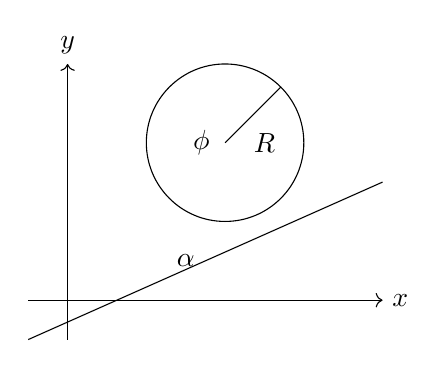
\begin{tikzpicture}
\draw[->] (-0.5,0) -- (4,0) node[right] {$x$};
\draw[->] (0,-0.5) -- (0,3) node[above] {$y$};
\draw (-0.5,-0.5) -- (4,1.5);
\draw (2,2) circle (1);
\draw (2,2) -- +(45:1);
\node at (1.5,0.5) {$\alpha$};
\node at (2.5,2) {$R$};
\node at (1.7,2) {$\phi$};
\end{tikzpicture}

Ohne ZBs würde die Lage der Scheibe durch 3 Koordinaten bestimmt,

ZB: $x_A, y_A, \phi$

2 holonome ZBs:

$x_A - R\phi \cos\alpha = 0$

$y_A - R\phi \sin\alpha = 0$
\end{EXA}

\begin{CONC}{CM-K25c-08-12}{Versionen der nicht-holonomen Zwangsbedingungen}
Nicht-holonome Zwangsbedingungen - Darunter versteht man alle ZB, die sich nicht auf Gleichungen der Form $f_j(q_1,...,q_M,t)=0$ zurückführen lassen, welche nur die generalisierten Koordinaten und die Zeit enthalten. (dabei ist M die maximal mögliche Zahl der generalisierten Koordinaten, $M=DN$ für N Teilchen in D Dimensionen).

Man unterscheidet zwei verschiedene Typen von nicht-holonomen ZB:

1) Ungleichungen:

Manche ZB lassen sich mathematisch nur als Ungleichungen formulieren.

\textbf{Beispiel:} Kleine Kugel rollt Oberfläche einer großen Kugel herunter:
ZB: $R(t) \geq R$

Ist die Geschwindigkeit der kleinen Kugel groß genug, verliert sie wegen ihrer Zentrifugalkraft beim Herunterfallen den Kontakt zur großen Kugel.

2) Nicht-integrable Zwangsbedingungen:

Darunter versteht man ZB der Form

\[f_j(q_1,...,q_M,\dot{q}_1,...,\dot{q}_M,t) = 0\]

die sich nicht durch geeignete Integration in holonome ZB der Form $h_j(q_1,...,q_M,t)=0$ umwandeln lassen.
\end{CONC}

\begin{CONC}{CM-K25c-08-13}{Holonomie und Exaktheit}
Betrachten wir zunächst eine \emph{holonome} Zwangsbedingung
\begin{equation}
  h_j\bigl(q_1,\dots,q_M,t\bigr)\;=\;0,
  \qquad j=1,\dots,k_{\mathrm{hol}} .
\end{equation}
Zeitliches Differenzieren liefert die (gleichwertige) Bedingung
\begin{equation}
  0 \;=\; \frac{\mathrm d}{\mathrm dt}\,
           h_j\bigl(q_1,\dots,q_M,t\bigr)
      \;=\;
      \sum_{i=1}^M 
        \frac{\partial h_j}{\partial q_i}\,\dot q_i
      + \frac{\partial h_j}{\partial t}
      \;\equiv\;
      f_j\bigl(\dot q_1,\dots,\dot q_M,t\bigr).
\end{equation}

% Differentialform
Multipliziert man mit $\mathrm dt$ und benutzt
$\mathrm dq_i = \dot q_i\,\mathrm dt$, erhält man die (Pfaffsche) 
Differentialform
\begin{equation}\label{eq:pfaff_hol}
  \sum_{i=1}^{M} a_{ji}\,\mathrm dq_i
  + a_{jt}\,\mathrm dt \;=\; 0, \qquad
  a_{ji}=\frac{\partial h_j}{\partial q_i},\quad
  a_{jt}=\frac{\partial h_j}{\partial t}.
\end{equation}

% Integrabilitätsbedingungen
Da die gemischten zweiten Ableitungen vertauschbar sind
(vorausgesetzt $h_j$ ist hinreichend glatt), gelten die
\emph{Integrabilitätsbedingungen}
\begin{align}
  \frac{\partial a_{ji}}{\partial q_k}
  &= \frac{\partial a_{jk}}{\partial q_i}
     \;=\;
     \frac{\partial^2 h_j}{\partial q_k\,\partial q_i},
     & i,k&=1,\dots,M,                                     \label{eq:int1}\\
  \frac{\partial a_{jt}}{\partial q_i}
  &= \frac{\partial a_{ji}}{\partial t}
     \;=\;
     \frac{\partial^2 h_j}{\partial q_i\,\partial t},
     & i&=1,\dots,M.                                       \label{eq:int2}
\end{align}
Die Pfaffsche Gleichung \eqref{eq:pfaff_hol} ist also \emph{exakt}, weil
sie als exaktes Differential $\mathrm d h_j$ entsteht.

% Nicht-integrable / nicht-holonome Zwangsbedingungen
In vielen Problemen treten jedoch \emph{nicht-holonome} (i.\,A.\, nicht
integrierbare) Zwangsbedingungen auf,
\begin{equation}\label{eq:pfaff_nh}
  \sum_{i=1}^{M} a_{ji}(q,t)\,\dot q_i
  + a_{jt}(q,t) \;=\; 0,
  \qquad j=1,\dots,k_{\mathrm{nh}},
\end{equation}
bzw.\ äquivalent in Differentialform
\(
  \sum_{i} a_{ji}\,\mathrm dq_i + a_{jt}\,\mathrm dt = 0 .
\)
Erfüllen die Koeffizienten $a_{ji},a_{jt}$ die
Integrabilitätsbedingungen \eqref{eq:int1}–\eqref{eq:int2} \emph{nicht},
so ist das Differential \emph{nicht exakt}.  

In manchen Fällen lässt sich durch Multiplikation mit einem
\emph{integrierenden Faktor} $\mu(q,t)\neq 0$
\[
  \mu\bigl(q,t\bigr)\,
  \Bigl(\sum_{i} a_{ji}\,\mathrm dq_i + a_{jt}\,\mathrm dt\Bigr)
  \;=\;
  \mathrm d H_j(q,t)
\]
eine exakte Form herstellen; gelingt dies jedoch nicht, kann
\eqref{eq:pfaff_nh} nicht auf eine holonome Bedingung
$H_j(q,t)=\text{const}$ integriert werden. Man spricht dann von einer
\emph{nicht-integrablen} Zwangsbedingung.
\end{CONC}

\begin{EXA}{CM-K25c-08-14}{Rollscheibe: Differentiale Zwangsbedingungen}
\textbf{1.\ Konfigurationskoordinaten}
Die Lage der Scheibe ist durch vier generalisierte Koordinaten vollständig
beschrieben
\[
  q \;=\; \bigl(x_A,\;y_A,\;\psi,\;\varphi\bigr)^{\mathrm T},
\]
\begin{itemize}
  \item $x_A,\;y_A$ – Koordinaten des Auflagepunktes $A$ in der Ebene,
  \item $\psi$ – Winkel zwischen der Bewegungsrichtung und der $x$-Achse,
  \item $\varphi$ – Rollwinkel der Scheibe um ihre Symmetrieachse.
\end{itemize}

\textbf{2.\ Kinematik des reinen Rollens}
Reines Abrollen ohne Gleiten liefert (Mechanik I, S.\,223)
\[
  V_{CM} \;=\; R\,\dot{\varphi},
\]
wobei die Geschwindigkeit des Schwerpunkts stets in die
Richtung $(\cos\psi,\,-\sin\psi)$ zeigt. Es folgt
\begin{align}
  \dot{x}_A &= R\,\dot{\varphi}\,\cos\psi,
  &
  \dot{y}_A &= -\,R\,\dot{\varphi}\,\sin\psi.
  \label{eq:velocities}
\end{align}

\textbf{3.\ Pfaffsche Zwangsbedingungen}
Die Geschwindigkeitsbeziehungen \eqref{eq:velocities} können als
differentiale (Pfaffsche) Zwangsbedingungen formuliert werden:
\begin{align}
  f_1 &:\; \boxed{\,dx_A - R\cos\psi\,d\varphi = 0\,},
  \label{eq:f1}\\[2mm]
  f_2 &:\; \boxed{\,dy_A + R\sin\psi\,d\varphi = 0\,}.
  \label{eq:f2}
\end{align}

\textbf{4.\ Integrabilitätsprüfung}

\paragraph{Zwangsbedingung \eqref{eq:f1}.}
Schreiben wir \eqref{eq:f1} als
\(
  \sum_{i=1}^{4} a_{1i}\,dq_i = 0
\)
mit den Koeffizienten
\[
  (a_{1x_A},\,a_{1y_A},\,a_{1\psi},\,a_{1\varphi})
  \;=\;
  (1,\,0,\,0,\,-R\cos\psi),
\]
so lautet die notwendige Integrabilitätsbedingung
\(
  \partial a_{1i}/\partial q_k
  =
  \partial a_{1k}/\partial q_i
\)
für alle Paare $(i,k)$.  
Für das Paar $(i,k)=(\psi,\varphi)$ ergibt sich
\[
  \frac{\partial a_{1\psi}}{\partial\varphi}
  \;=\; 0
  \;\neq\;
  \frac{\partial a_{1\varphi}}{\partial\psi}
  \;=\;
  R\sin\psi,
\]
womit \eqref{eq:f1} \emph{nicht integrierbar} ist.

\paragraph{Zwangsbedingung \eqref{eq:f2}.}
Für
\[
  (a_{2x_A},\,a_{2y_A},\,a_{2\psi},\,a_{2\varphi})
  \;=\;
  (0,\,1,\,0,\,R\sin\psi)
\]
liefert das Paar $(\psi,\varphi)$ den Widerspruch
\[
  \frac{\partial a_{2\psi}}{\partial\varphi}=0
  \;\neq\;
  \frac{\partial a_{2\varphi}}{\partial\psi}=R\cos\psi,
\]
sodass auch \eqref{eq:f2} nicht integrierbar ist.

\textbf{5.\ Kein integrierender Faktor für \eqref{eq:f1}}
Sei hypothetisch $\mu=\mu(q)\neq0$ so, dass $\mu\,f_1$ exakt wäre.
Notwendig wäre dann
\[
  \frac{\partial(\mu a_{1i})}{\partial q_k}
  \;=\;
  \frac{\partial(\mu a_{1k})}{\partial q_i}
  \quad\forall\,i,k.
\]
Aus dem Paar $(i,k)=(x_A,\psi)$ folgt
$\partial\mu/\partial\psi = 0$ (also $\mu$ unabhängig von $\psi$),
während das Paar $(\psi,\varphi)$ verlangt
\(
  \mu R\sin\psi = 0
\),
was bei beliebigem $\psi$ nur für $\mu\equiv0$ erfüllbar ist.
Ein nicht-trivialer integrierender Faktor existiert somit nicht.

\textbf{6.\ Schlussfolgerung}
Die Pfaffschen Gleichungen \eqref{eq:f1}–\eqref{eq:f2} verletzen die
Integrabilitätsbedingungen und besitzen keinen integrierenden Faktor.
Die Abrollbedingungen sind daher \emph{nicht holonom};
sie lassen sich nicht auf rein
koordinatenabhängige Gleichungen
\(
  H_j\bigl(x_A,y_A,\psi,\varphi\bigr)=\text{const.}
\)
zurückführen.
\end{EXA}

\begin{CONC}{CM-K25c-08-15}{Zwangkräfte in Newton'schen Bewegungsgleichungen}
\textbf*{Ziel}
Bestimmung der \emph{Zwangkräfte} (Reaktions- oder Führungskräfte) 
für \underline{holonome} Zwangsbedingungen innerhalb der klassisch
newton’schen Formulierung.

%--------------------------------------------------------------------
\textbf*{Gegeben}
\begin{itemize}
  \item $N$ Massenpunkte in $D$ Dimensionen $\;\Longrightarrow\; M=DN$
        kartesische Koordinaten\,(*)  
        \[
          \bigl\{\,x_{i}^{(\alpha)}\bigr\}_{\substack{i=1,\dots,N\\\alpha=1,\dots,D}},
          \quad
          \text{kurz } 
          (q_1,\dots,q_M).
        \]
  \item $k$ unabhängige \emph{holonome} Zwangsbedingungen
        \[
          f_j\bigl(q_1,\dots,q_M,t\bigr)=0,
          \qquad j=1,\dots,k .
        \]
\end{itemize}
Damit verbleiben $n=M-k$ unabhängige generalisierte Koordinaten.

%--------------------------------------------------------------------
\textbf*{Methode in drei Schritten}

\textbf{1.\ Wahl unabhängiger Koordinaten}
\[
  q_\mu = q_\mu(q_1,\dots,q_n,t), 
  \qquad \mu = 1,\dots,M .
\]
In kartesischer Form (hier $D=3$) erhält man
\[
  \vec r_i = 
  \begin{pmatrix}
    x_i(q_1,\dots,q_n,t)\\[2pt]
    y_i(q_1,\dots,q_n,t)\\[2pt]
    z_i(q_1,\dots,q_n,t)
  \end{pmatrix},
  \qquad
  i=1,\dots,N .
\]

\textbf{2.\ Newtonsche Bewegungsgleichungen}
\[
  m_i\,\ddot{\vec r}_i
  \;=\;
  \vec F_i^{\text{(ext)}}(q,\dot q,t)
  \;+\;
  \vec Z_i(q,\dot q,t),
  \qquad i=1,\dots,N .
\]
\emph{Unbekannt} sind hier die $M=DN$ Komponenten der
Zwangkräfte~$\vec Z_i$.

Sobald die Beschleunigungen $\ddot{\vec r}_i$
aus den Bewegungsgleichungen bestimmt sind, folgt
\[
  \vec Z_i 
  \;=\;
  m_i\,\ddot{\vec r}_i - \vec F_i^{\text{(ext)}} .
\]

\textbf{3.\ Eliminieren der Zwangkräfte}
\begin{itemize}
  \item Unbekannte Größen  
        \[
          \underbrace{q_1,\dots,q_{n}}_{\text{Koordinaten}}
          \quad\cup\quad
          \underbrace{Z_{1}^{(1)},\dots,Z_{N}^{(D)}}_{\text{Zwangkräfte}}
          \;\Longrightarrow\;
          (M-k)+M = 2M-k \text{ Unbekannte.}
        \]
  \item Gleichungen  
        \[
          \text{Newton: } M,\qquad
          \text{ZB + deren Zeitd.}: 2k
          \quad\Longrightarrow\quad
          M+2k \text{ Gleichungen.}
        \]
        Für holonome ZB ($k$ unabhängig) lassen sich $k$ der 
        $Z$-Komponenten rein algebraisch beseitigen, sodass exakt
        $M$ Gleichungen für die $M$ Unbekannten verbleiben.
  \item Ergebnis: Ein geschlossenes Differentialgleichungssystem
        \[
          \bigl\{\,q_\alpha(t)\bigr\}_{\alpha=1}^{n}
        \]
        ohne explizite Zwangkräfte.
\end{itemize}

\medskip
\noindent
(*) \emph{Indexkonvention:} $i$ zählt die Teilchen $(1,\dots,N)$,
$\alpha$ die kartesischen Komponenten $(1,\dots,D)$,
$q_1,\dots,q_M$ sind die vollständigen (u.\,U.\ abhängigen)
Koordinaten, $q_1,\dots,q_n$ die unabhängigen.
\end{CONC}

\begin{EXA}{CM-K25c-08-16}{Teilchen auf Kreiskegel}
\begin{center}
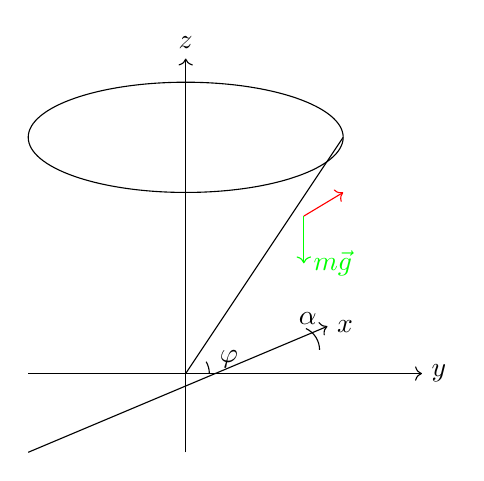
\begin{tikzpicture}[scale=1]
  % Achsen
  \draw[->] (-2,0) -- (3,0) node[right] {$y$};
  \draw[->] (0,-1) -- (0,4) node[above] {$z$};
  \draw[->] (-2,-1) -- (1.8,0.6) node[right] {$x$};
  % Kegel
  \draw (0,0) -- (2,3);
  \draw (0,3) ellipse (2cm and 0.7cm);
  \draw[dashed] (0,0) -- (2,0);
  % Winkel
  \draw (0.3,0) arc (0:30:0.3);
  \node at (0.55,0.18) {$\varphi$};
  \draw (1.7,0.3) arc (0:65:0.3);
  \node at (1.55,0.7) {$\alpha$};
  % Kräfte
  \draw[red,->] (1.5,2) -- (2,2.3);
  \draw[green,->] (1.5,2) -- (1.5,1.4) node[right] {$m\vec g$};
\end{tikzpicture}
\end{center}

\textbf{Geometrische Daten}\\
Ein Teilchen der Masse $m$ bewegt sich auf der Innenseite eines
Kreiskegels mit Halbwinkel $\alpha$ unter der Wirkung einer konstanten
Erdbeschleunigung $\vec g = -g\,\vec e_z$.  
Zylinderkoordinaten $(S,\varphi,z)$ sind geeignet; die
holonome Zwangsbedingung lautet
\[
  f(S,z)=S-z\tan\alpha=0
  \;\Longrightarrow\;
  z = S\cot\alpha .
\]

\textbf{Schritt 1 – unabhängige Koordinaten}\\
Wähle $q_1=S$ und $q_2=\varphi$.
Die kartesischen Orts­komponenten ergeben sich zu
\[
  \begin{pmatrix} x \\ y \\ z \end{pmatrix} =
  \begin{pmatrix}
    S\cos\varphi \\[2pt]
    S\sin\varphi \\[2pt]
    S\cot\alpha
  \end{pmatrix}.
\]

\textbf{Schritt 2 – Newtonsche Gleichungen mit Zwangkräften}\\
\[
  m\!
  \begin{pmatrix}
    \ddot x\\ \ddot y\\ \ddot z
  \end{pmatrix}
  =
  \underbrace{%
  \begin{pmatrix}
    0\\[2pt] 0\\[2pt] -\,mg
  \end{pmatrix}}_{\vec F^{\text{(ext)}}}
  +
  \underbrace{%
  \begin{pmatrix}
    Z_x\\ Z_y\\ Z_z
  \end{pmatrix}}_{\vec Z}.
\]
Mit
\[
  \dot x = \dot S\cos\varphi - S\dot\varphi\sin\varphi,\qquad
  \dot y = \dot S\sin\varphi + S\dot\varphi\cos\varphi,\qquad
  \dot z = \dot S\cot\alpha,
\]
folgen die Beschleunigungen
\begin{align}
  \ddot x &= \ddot S\cos\varphi - 2\dot S\dot\varphi\sin\varphi
             - S\dot\varphi^{2}\cos\varphi - S\ddot\varphi\sin\varphi,
             &(1)\nonumber\\[2pt]
  \ddot y &= \ddot S\sin\varphi + 2\dot S\dot\varphi\cos\varphi
             - S\dot\varphi^{2}\sin\varphi + S\ddot\varphi\cos\varphi,
             &(2)\nonumber\\[2pt]
  \ddot z &= \ddot S\cot\alpha. &(3)\nonumber
\end{align}
Damit lauten die Komponenten­gleichungen
\begin{align}
  m\bigl(\ddot S\cos\varphi - 2\dot S\dot\varphi\sin\varphi
        - S\dot\varphi^{2}\cos\varphi - S\ddot\varphi\sin\varphi\bigr) &= Z_x, \tag{A}\\[2pt]
  m\bigl(\ddot S\sin\varphi + 2\dot S\dot\varphi\cos\varphi
        - S\dot\varphi^{2}\sin\varphi + S\ddot\varphi\cos\varphi\bigr) &= Z_y, \tag{B}\\[2pt]
  m\bigl(\ddot S\cot\alpha\bigr) - mg &= -\,Z_z. \tag{C}
\end{align}
(Die Form \eqref{C} wählt $Z_z$ positiv nach oben.)

\textbf{Schritt 3 – Eliminieren der Zwangkräfte}\\
Die Reaktionskraft $\vec Z$ steht stets senkrecht zur Kegeloberfläche.  
Aus der Draufsicht (radiale Richtung)
\[
  \begin{pmatrix} Z_x\\ Z_y \end{pmatrix}
    = -\,Z_\perp\!\begin{pmatrix}\cos\varphi\\ \sin\varphi\end{pmatrix},
\]
folgt
\[
  Z_y\cos\varphi - Z_x\sin\varphi = 0. \tag{D}
\]
Aus der Seitenansicht (Neigungswinkel $\alpha$) erhält man
\[
  Z_z = Z_\perp\tan\alpha
  \;\Longrightarrow\;
  Z_z\cos\varphi + Z_x\tan\alpha = 0. \tag{E}
\]

\textbf{Kombination der Gleichungen}\\
\begin{enumerate}
  \item[(i)]  $(\text{A})\sin\varphi - (\text{B})\cos\varphi$
              unter Verwendung von \eqref{D} liefert
              \[
                2\dot S\,\dot\varphi + S\ddot\varphi = 0. \tag{1}
              \]
  \item[(ii)] $(\text{A})\tan\alpha + (\text{C})\cos\varphi$
              und Bedingung \eqref{E} ergeben
              \[
                (\tan\alpha + \cot\alpha)\,\ddot S
                - S\dot\varphi^{2}\tan\alpha + g = 0. \tag{2}
              \]
\end{enumerate}
Die zwei Differential­gleichungen \eqref{1} und \eqref{2} enthalten nur
die unabhängigen Koordinaten $S(t)$ und $\varphi(t)$;
die Zwangkräfte sind eliminiert.  
Nach Bestimmung von $S(t),\varphi(t)$ können $Z_x,Z_y,Z_z$ aus
(A)–(C) rückwärts berechnet werden.

\textbf{Fazit}\\
Das rein newton’sche Vorgehen erfordert
\emph{zuerst} das Einführen und
\emph{anschließende} Eliminieren der unbekannten Zwangkräfte – ein
umständlicher Prozess.  
Die Frage, ob man die Bewegungsgleichungen der unabhängigen Koordinaten
direkt (ohne $\vec Z$) erhält, wird von der Lagrange’schen Formulierung
beantwortet (D’Alembert–Lagrange-Prinzip).
\end{EXA}

\subsection{Kanonische Transformationen und Invarianten}

\begin{CONC}{CM-K25c-17-01}{Punkttransformationen}
In der Lagrange-Mechanik kann man beliebige Punkttransformationen ausführen (siehe Kapitel 3.2. Forminvarianz der Lagrangegleichungen, S. 55). Dabei definiert man neue generalisierte Koordinaten

\[Q_i = Q_i(q_1,...,q_n,t), \quad i=1,...n\]

(wir ändern hier die Notation auf S.55: $q \rightarrow Q$).
Jeder Punkt $q=(q_1,...,q_n)$ des Konfigurationsraumes geht dabei in einen neuen Punkt $Q=(Q_1,...,Q_n)$ über. In Kapitel 3.2. haben wir gezeigt: die Lagrangegleichungen sind forminvariant unter solchen Punkttransformationen:

mit \[L'(Q,\dot{Q},t) = L(q(Q,t),\dot{q}(Q,\dot{Q},t),t)\]

\[\Rightarrow \frac{d}{dt}\frac{\partial L'}{\partial \dot{Q_i}} - \frac{\partial L'}{\partial Q_i} = 0.\]

Da $L'(Q,\dot{Q},t)$ i.A. jedoch eine andere Funktion der neuen Variablen ist als $L(q,\dot{q},t)$ der alten Variablen, ändert sich jedoch der explizite Ausdruck der Lagrangegleichungen bei Punkttransformationen.

Welche Änderungen gibt es bei Punkttransformationen im Hamilton-Formalismus?

Um diese Frage zu beantworten, müssen wir die neuen Kanonischen Impulse $P_i$ berechnen!


\begin{align*}
P_i = \frac{\partial L}{\partial \dot{q}_i} = \sum_{j=1}^n \frac{\partial L}{\partial \dot{q}_j} \frac{\partial \dot{q}_j}{\partial \dot{q}_i} = \sum_{j=1}^n p_j \frac{\partial \dot{q}_j}{\partial \dot{q}_i}
\end{align*}

$p_j = $ alte kanonische Impulse

wegen $\frac{\partial \dot{q}_j}{\partial \dot{q}_i} = \frac{\partial q_j}{\partial q_i}$ (siehe S. 56)

\begin{equation*}
\Rightarrow P_i = \sum_{j=1}^n p_j \frac{\partial q_j}{\partial q_i} : \text{ Transformation der kanonischen Impulse bei Punkttransformationen}
\end{equation*}

Wir definieren nun die neue Hamiltonfunktion
\begin{equation*}
H'(Q,P,t) = \sum_{i=1}^n \dot{Q}_i(Q,P,t)P_i - L'(Q,\dot{Q}(Q,P,t),t)
\end{equation*}

Wegen der Forminvarianz der Lagrangegleichungen bei Punkttransformationen folgt dann analog zur Herleitung der Hamiltonschen Bewegungsgleichungen aus Lagrange'L auf S. 157:

\begin{align*}
\dot{Q}_i &= \frac{\partial H'}{\partial P_i}, & P_i = -\frac{\partial H'}{\partial Q_i}
\end{align*}

d.h. Punkttransformationen lassen auch die Hamiltonschen Bewegungsgleichungen forminvariant.
\end{CONC}

\begin{CONC}{CM-K25c-17-02}{Kanonische Transformationen}
Da im Hamiltonformalsmus q und p völlig gleichberechtigt sind, können wir auch allgemeinere Transformationen betrachten, die Koordinaten und Impulse durcheinandermischen:


Kanonische Transformation:\\
Eine Transformation der Form
\begin{align*}
q_i &\to Q_i = Q_i(q_1 \ldots q_n, p_1 \ldots p_n, t)\\
p_i &\to P_i = P_i(q_1 \ldots q_n, p_1 \ldots p_n, t)
\end{align*}
heißt kanonisch, wenn aus $\dot{q}_i = \frac{\partial H}{\partial p_i}$, $\dot{p}_i = -\frac{\partial H}{\partial q_i}$ folgt, dass mit einer geeigneten neuen Hamilton-Funktion $H'(Q,P,t)$ die Form der Hamilton-Gleichungen invariant bleibt, d.h.
\begin{align*}
\dot{Q}_i &= \frac{\partial H'}{\partial P_i}, & \dot{P}_i = -\frac{\partial H'}{\partial Q_i}
\end{align*}
\end{CONC}

\begin{CONC}{CM-K25c-17-03}{Punkttransformationen sind Kanonische Transformationen}
Die unter a) diskutierten Punkttransformationen sind z.B. kanonisch. Es gibt aber auch andere kanonische Transformationen die die Koordinaten und Impulse wirklich durcheinander mischen. Nicht jede Transformation $q_i \to Q_i(q,p,t)$, $p_i \to P_i(q,p,t)$ ist jedoch automatisch kanonisch. Im Folgenden suchen wir Kriterien dafür, dass eine Trafo kanonisch ist, und entwickeln dabei auch eine Methode kanonische Trafos explizit zu konstruieren.
\end{CONC}

\begin{CONC}{CM-K25c-17-04}{Erzeugung von kanonischen Transformationen}
Wir wissen dass die Hamiltonschen Gleichungen aus dem Prinzip der stationären Wirkung folgen: (siehe S.169)

\begin{align*}
\delta \left[\int_{t_1}^{t_2} dt\left(\sum_{i=1}^n p_i\dot{q}_i - H\right)\right] &= 0\\
\text{mit } \delta q_i(t_1) = \delta q_i(t_2) &= 0
\end{align*}
\[\Rightarrow \dot{q}_i = \frac{\partial H}{\partial p_i}, \quad \dot{p}_i = -\frac{\partial H}{\partial q_i} \quad (1)\]

Wir führen nun neue Koordinaten und Impulse ein,
\[Q_i = Q_i(q,p,t), \quad P_i = P_i(q,p,t) \quad (2)\]

Wenn diese Transformation kanonisch ist, dann muss es eine neue Hamiltonfunktion $H'$ geben so dass
\[\dot{Q}_i = \frac{\partial H'}{\partial P_i}, \quad \dot{P}_i = -\frac{\partial H'}{\partial Q_i} \quad (3)\]

Das ist sicherlich der Fall wenn für die neuen Koordinaten, Impulse und die neue Hamiltonfunktion unter dem Prinzip der stationären Wirkung gilt:

\begin{align*}
\delta \left[\int_{t_1}^{t_2} dt\left(\sum_{i=1}^n P_i\dot{Q}_i - H'\right)\right] &= 0\\
\text{mit } \delta Q_i(t_1) = \delta Q_i(t_2) &= 0
\end{align*}
\[\Rightarrow \dot{Q}_i = \frac{\partial H'}{\partial P_i}, \quad \dot{P}_i = -\frac{\partial H'}{\partial Q_i}\]
\end{CONC}

\begin{CONC}{CM-K25c-17-05}{Eindeutige Bestimmung der Beweungungsgleichung durch Transformationsgleichung}
Andererseits bestimmen die Transformationsgleichungen 
\[Q_i = Q_i(q,p,t), \quad P_i = P_i(q,p,t) \quad (2)\]
zusammen mit den ursprünglichen Hamiltongleichungen 
\[ \dot{p}_i = -\frac{\partial H}{\partial q_i} \quad (1)\]
eindeutig die Bewegungsgleichungen von $Q_i$ und $P_i$.
\end{CONC}

\begin{CONC}{CM-K25c-17-06}{Hinreichende Bedingung für Transformationsverhalten von Hamiltonfunktion}
Ein hinreichende Bedingung dafür dass letztere von der Form
\[\dot{Q}_i = \frac{\partial H'}{\partial P_i}, \quad \dot{P}_i = -\frac{\partial H'}{\partial Q_i} \quad (3)\]
sind ist:

\[\sum_{i=1}^n p_i\dot{q}_i - H = \sum_{i=1}^n P_i\dot{Q}_i - H' + \frac{d}{dt}F_1(q,Q,t) \quad (4)\]

wobei $F_1$ eine beliebige Funktion der $q_i, Q_i$ und $t$ ist.Das folgt aus der Tatsache, dass dann die neue Hamiltonfunktion mit den neuen generalisierten Koordinaten das Prinzip der stationären Wirkung erfüllt:

\begin{align*}
\delta\left[\int_{t_1}^{t_2} dt\left(\sum_{i=1}^n P_i\dot{Q}_i - H'\right)\right] &= \delta\left[\int_{t_1}^{t_2} dt\left(\sum_{i=1}^n p_i\dot{q}_i-H\right)\right] - \delta\left[\int_{t_1}^{t_2} dt\frac{d}{dt}F_1(q,Q,t)\right]\\
&= -\delta F_1(q(t_2),Q(t_2),t_2) + \delta F_1(q(t_1),Q(t_1),t_1) = 0
\end{align*}
\end{CONC}

\begin{DEF}{CM-K25c-17-07}{erzeugende der kanonischen Transformation (differentielle Form)}
In differenzieller Form ist die Bedingung:
\[\sum_{i=1}^n p_i\dot{q}_i - H = \sum_{i=1}^n P_i\dot{Q}_i - H' + \frac{d}{dt}F_1(q,Q,t) \quad (4)\]
gegeben durch 
\[dF_1(q,Q,t) = \sum_{i=1}^n (p_i dq_i - P_i dQ_i) + (H'-H)dt\]

\[\Rightarrow \frac{\partial F_1(q,Q,t)}{\partial q_i} = p_i, \quad \frac{\partial F_1(q,Q,t)}{\partial Q_i} = -P_i, \quad \frac{\partial F_1(q,Q,t)}{\partial t} = H'-H\]

Man nennt $F_1(q,Q,t)$ die "Erzeugende der Kanonischen Transformation".
\end{DEF}

\begin{CONC}{CM-K25c-17-08}{Eindeutige Bestimmung der Transformationgleichung aus Erzeugende}
Wenn $F_1(q,Q,t)$ bekannt ist, lassen sich die Transformationsgleichungen eindeutig bestimmen: Durch Auflösen von $p_i = \frac{\partial F_1(q,Q,t)}{\partial q_i}$ erhält man die neuen Koordinaten $Q_i = Q_i(q,p,t)$, und dann durch Auflösen von $P_i = -\frac{\partial F_1(q,Q,t)}{\partial Q_i}$ die restlichen Gleichungen $P_i = P_i(q,p,t)$. Schließlich erhält man die neue Hamiltonfunktion aus
\[H'(Q,P,t) = H(q(Q,P,t),p(Q,P,t),t) + \left.\frac{\partial F_1(q,Q,t)}{\partial t}\right|_{q=q(Q,P,t)}\]

Man beachte dass die Hamiltonfunktion nur dann wie ein Skalar transformiert wenn die Erzeugende nicht explizit von der Zeit abhängt. Im Gegensatz dazu transformiert die Lagrangefunktion bei beliebigen Punkttrafos immer wie ein Skalar, siehe S. 55.
\end{CONC}

\begin{CONC}{CM-K25c-17-10}{Alternative unabhängige Variablen}
Bisher haben wir zur Konstruktion Kanonischer Transformationen benutzt dass die Existenz einer Funktion $F_1(q,Q,t)$ mit
\[dF_1 = \left(\sum_{i=1}^n p_i dq_i - H dt\right) - \left(\sum_{i=1}^n P_i dQ_i - H' dt\right)\]
eine hinreichende Bedingung dafür ist dass die entsprechende Transformation $Q_i = Q_i(q,p,t)$, $P_i = P_i(q,p,t)$ Kanonisch ist.

Es gibt jedoch auch andere Möglichkeiten zur Erzeugung Kanonischer Trafos, denn im Hamiltonformalism sind Koordinaten und Impulse gleichberechtigt: An den Variablen $q_1,..,q_n,Q_1,..,Q_n,p_1,..,p_n,P_1,..,P_n$ können wir daher beliebig 2n als unabhängig ansehen, während die anderen 2n auf Grund der Transformationsgleichungen als abhängig betrachtet werden müssen. Der Übergang zu neuen unabhängigen Variablen erfolgt durch Legendre-Trafo. Da die Erzeugenden jeweils von einem alten und einem neuen Variablen-Satz abhängen müssen, gibt es neben $F_1(q,Q)$ noch 3 weitere Möglichkeiten:
\end{CONC}

\begin{CONC}{CM-K25c-17-11}{$(q,P)$ unabhängige Variablen}
Erzeugende: $F_2(q,P,t) = F_1(q,Q(q,P,t),t) + \sum_{i=1}^n P_i Q_i(q,P,t)$

$\Rightarrow$ $dF_2 = dF_1 + \sum_i (P_i dQ_i + Q_i dP_i)$

$= \sum_i (p_i dq_i + Q_i dP_i) - (H'-H)dt$

$\Rightarrow \frac{\partial F_2}{\partial q_i} = p_i$, $\frac{\partial F_2}{\partial P_i} = Q_i$, $\frac{\partial F_2}{\partial t} = H'-H$.
\end{CONC}

\begin{CONC}{CM-K25c-17-12}{$(p,Q)$ unabhängige Variablen}
$F_3(p,Q,t) = F_1 - \sum_i q_i p_i$

$\Rightarrow dF_3 = \sum_{i=1}^n (-q_i dp_i - P_i dQ_i) + (H'-H)dt$

$\Rightarrow \frac{\partial F_3}{\partial p_i} = -q_i$, $\frac{\partial F_3}{\partial Q_i} = -P_i$, $\frac{\partial F_3}{\partial t} = H'-H$
\end{CONC}

\begin{CONC}{CM-K25c-17-13}{$(p,P)$ unabhängige Variablen}
$F_4(p,P,t) = F_3 + \sum_i P_i Q_i$

$\Rightarrow dF_4 = \sum_{i=1}^n (-q_i dp_i + Q_i dP_i) + (H'-H)dt$

$\Rightarrow \frac{\partial F_4}{\partial p_i} = -q_i$, $\frac{\partial F_4}{\partial P_i} = Q_i$, $\frac{\partial F_4}{\partial t} = H'-H$
\end{CONC}

\begin{CONC}{CM-K25c-17-14}{Funktionen erzeugen kanonische Transformationen}
Daß die Funktionen $F_1, F_3, F_4$ Kanonische Transformationen erzeugen folgt wie auf S. 160 aus dem Hamilton'schen Prinzip, wobei man allerdings bei der Behandlung der Randterme beachten muss dass die Variation der Impulse $\delta p_i(t_{1,2})$ und $\delta P_i(t_{1,2})$ an den Rändern nicht verschwindet - dennoch verschwinden die Beiträge aller Randterme nach geeigneter partieller Integration (siehe z.B. Goldstein, Mechanik II, S. 236).

Alternativ kann man auch direkt nachrechnen dass die obigen Trafos in der Tat kanonisch sind:

Ausgangspunkt: $\dot{q}_i = \frac{\partial H}{\partial p_i}$, $\dot{p}_i = -\frac{\partial H}{\partial q_i}$

mit Transformationsgleichungen:
$Q_i = Q_i(q,p,t)$, $P_i = P_i(q,p,t)$
Zu zeigen: mit $H' = H + \frac{\partial F}{\partial t}$, wobei $F = F_1, F_2, F_3, F_4$ gilt,

gilt: $\dot{Q}_i = \frac{\partial H'}{\partial P_i}$, $\dot{P}_i = -\frac{\partial H'}{\partial Q_i}$
\end{CONC}

\begin{CONC}{CM-K25c-17-15}{Invarianz der fundamentalen Poisson-Klammer-Relationen bei Kanonischen Trafos}
Invarianz der fundamentalen Poisson-Klammer-Relationen bei Kanonischen Trafos
\[
\{Q_i, P_j\} = \sum_k \left(\frac{\partial Q_i}{\partial q_k}\frac{\partial P_j}{\partial p_k} - \frac{\partial P_j}{\partial q_k}\frac{\partial Q_i}{\partial p_k}\right) = \delta_{ij} = \{q_i, p_j\}
\]
\end{CONC}

\begin{EXA}{CM-K25c-17-16}{Zeitunabhängige Kanonische Trafos}
Für alle 4 Typen von Kanonischen Transformationen gilt:
Sind die Transformationsgleichungen nicht explizit von der Zeit abhängig, so ist $H' = H$. Eine Transformation $Q_i = Q_i(q,p)$, $P_i = P_i(q,p)$ ist genau dann Kanonisch wenn

\[\sum_{i=1}^n (p_i\dot{q}_i - P_i\dot{Q}_i) = \frac{dF}{dt}\]

mit einer geeigneten Funktion F.

\[\sum_{i=1}^n (p_idq_i - P_idQ_i) = dF\]
\end{EXA}

\begin{EXA}{CM-K25c-17-17}{Identische Trafo}
\[F_2(q,P) = \sum_{i=1}^n q_iP_i \Rightarrow p_i = \frac{\partial F_2}{\partial q_i} = P_i, \quad Q_i = \frac{\partial F_2}{\partial P_i} = q_i\]
\end{EXA}

\begin{EXA}{CM-K25c-17-18}{Punkttransformation}
\[F_2(q,P,t) = \sum_{i=1}^n \phi_i(q_1,...,q_n,t)P_i\]
\[\Rightarrow \quad Q_i = \frac{\partial F_2}{\partial P_i} = \phi_i(q_1...q_n,t)\]
\[p_i = \frac{\partial F_2}{\partial q_i} = \sum_j \frac{\partial \phi_j}{\partial q_i}P_j = \sum_j \frac{\partial Q_j}{\partial q_i}P_j\]
\end{EXA}

\begin{EXA}{CM-K25c-17-19}{Vertauschung von Koordinaten und Impulsen}
\[F_1(q,Q) = \sum_{i=1}^n q_iQ_i \Rightarrow p_i = \frac{\partial F_1}{\partial q_i} = Q_i, \quad P_i = -\frac{\partial F_1}{\partial Q_i} = -q_i\]
\end{EXA}

\begin{EXA}{CM-K25c-17-20}{Bogoliubov-Transformation}
\[F_2(q,P) = \frac{\tanh\gamma(P^2-q^2)}{2} + \frac{1}{\cosh\gamma}qP, \quad \gamma \text{ beliebig}\]

\[\Rightarrow p = \frac{\partial F_2}{\partial q} = -\tanh\gamma q + \frac{1}{\cosh\gamma}P \Rightarrow P = \cosh\gamma p + \sinh\gamma q\]

\[Q = \frac{\partial F_2}{\partial P} = \tanh\gamma P + \frac{1}{\cosh\gamma}q\]
\[= \tanh\gamma(\cosh\gamma p + \sinh\gamma q) + \frac{1}{\cosh\gamma}q\]
\[= \sinh\gamma p + \frac{\sinh^2\gamma}{\cosh\gamma}q\]
\[= \sinh\gamma p + \cosh\gamma q\]

Mit $M = \cosh t$, $N = \sinh t$ Bogoliubov-Trafo somit:

\[
\begin{pmatrix} Q \\ P \end{pmatrix} = 
\begin{pmatrix} M & N \\ N & M \end{pmatrix}
\begin{pmatrix} q \\ p \end{pmatrix}, \quad M^2 - N^2 = \cosh^2 t - \sinh^2 t = 1
\]
\end{EXA}

\begin{PROP}{CM-K25c-17-21}{Hamiltonsche Zeitentwicklung aus Kanonische Trafo}
Wir betrachten die Erzeugende 
$$T_1(q,P,t) = q\cdot P + H(q,P,t)dt$$ 
wobei $dt = t'-t$ ein infinitesimales Zeitintervall ist, und $H(q,P,t)$ die Hamiltonfunktion (aufgefasst als Funktion von $q,P$). Dann gilt

\[
P = \frac{\partial T}{\partial q} = P + \frac{\partial H}{\partial q}dt = P - \dot{P}dt
\]

\[
Q = \frac{\partial T}{\partial P} = q + \frac{\partial H}{\partial P}dt = q + \dot{q}dt
\]

Da neuen Variablen sind also die "zeitentwickelte" Alten,

\[
Q(t) = q(t) + \dot{q}(t)dt \approx q(t+dt) = q(t')
\]

\[
P(t) = p(t) + \dot{p}(t)dt \approx p(t+dt) = p(t')
\]

d.h. infinitesimale Zeittrasfomationen, in denen $q(t+dt)$, $p(t+dt)$ gemäß den Hamiltonschen Bewegungsgleichungen aus $q(t)$, $p(t)$ hervorgehen, besitzen eine Erzeugende $T_1(q,P,t)$ und sind somit Kanonische Transformationen.

Da sich die Hamiltonsche Zeitentwicklung über ein endliches Zeitintervall $t-t_0$ durch Hintereinanderausführung von infinitesimalen Trafos zusammensetzen lässt, gilt:

Die Hamiltonsche Zeitentwicklung eines mechanischen Systems von Anfangswerten $q(t_0), p(t_0)$ zu Endwerten $q(t) = Q$, $p(t) = P$ ist eine Kanonische Transformation, die von einem kontinuierlichen Parameter $t$ abhängt.


Die Erzeugende $T_2(q_1..q_n, P_1..P_n,t)$ der Kanonischen Trafo ist durch die Lösung der Hamilton-Jacobi-Gleichung gegeben.
\end{PROP}

\begin{DEF}{CM-K25c-18-01}{Kanonische Invarianten}
Darunter versteht man Zusammenhänge zwischen Observablen oder auch Eigenschaften des von den $q_i$ und $p_i$ aufgespannten $2n$-dimensionalen Phasenraums, die sich bei Kanonischen Transformationen nicht ändern.
\end{DEF}

\begin{EXA}{CM-K25c-18-02}{Hamiltonsche Gleichungen als Kanonische Invarianten}
Hamiltonsche Gleichungen. (Dies ist trivial, denn Kanonische Trafos sind ja gerade so definiert dass sie die Form der Hamiltonschen Gleichungen nicht ändern.)
\end{EXA}

\begin{EXA}{CM-K25c-18-03}{Poisson-Klammern-Relationen als Kanonische Invarianten}
Alle Poissonklammer-Relationen bleiben bei Kanonischen Transformationen erhalten. In Formeln heißt das folgendes:

Gegeben seien beliebige Observablen $F(q,p,t)$, $G(q,p,t)$
\[
\{q_i, p_j\} = \delta_{ij}, \quad \{q_i, q_j\} = 0 = \{p_i, p_j\}
\]

Kanonische Trafo: $Q_i = Q_i(q,p,t)$, $P_i = P_i(q,p,t)$

\[
F'(Q,P,t) = F(q(Q,P,t), p(Q,P,t), t)
\]
\[
G'(Q,P,t) = G(q(Q,P,t), p(Q,P,t), t)
\]

Dann gilt: $$\{F, G\} = \sum_i \left(\frac{\partial F}{\partial q_i} \frac{\partial G}{\partial p_i} - \frac{\partial G}{\partial q_i} \frac{\partial F}{\partial p_i}\right)$$
\[
= \sum_i \left(\frac{\partial F'}{\partial Q_i} \frac{\partial G'}{\partial P_i} - \frac{\partial G'}{\partial Q_i} \frac{\partial F'}{\partial P_i}\right) = \{F', G'\}
\]
\end{EXA}

\begin{EXA}{CM-K25c-18-04}{Spezielle Poisson-Klammern-Relationen als Kanonische Invarianten}
Die fundamentalen Poisson-Klammer-Relationen bleiben bei Kanonischen Transformationen erhalten.

$$\{Q_i, P_j\} = \sum_k \left(\frac{\partial Q_i}{\partial q_k} \frac{\partial P_j}{\partial p_k} - \frac{\partial P_j}{\partial q_k} \frac{\partial Q_i}{\partial p_k}\right) = \{q_i, p_j\} = \delta_{ij}$$

$$\{Q_i, Q_j\} = \{q_i, q_j\} = 0$$

$$\{P_i, P_j\} = \{p_i, p_j\} = 0$$

An diesem Punkt kann man so am einfachsten testen, ob eine gegebene Transformation Kanonisch ist oder nicht.
\end{EXA}

\begin{EXA}{CM-K25c-18-05}{Phasenvolumen als Kanonische Invarianten}
Das Volumen des Phasenraumes ändert sich bei Kanonischen Transformationen nicht.


Dabei ist der Phasenraum definiert als der 2n-dimensionale, nicht-gekrümmte Raum, dessen 2n kartesische Achsen den Kanonisch konjugierten Variablen $q_1...q_n, p_1...p_n$ entsprechen.

Ein gegebenes Volumen $V_{2n} = \int dq_1 \int dq_2 ... \int dq_n \int dp_1 ... \int dp_n$ 
des alten Phasenraumes ändert bei einer Kanonischen Transformation 
zwar seine Form, aber nicht sein Volumen, d.h.

\[
V'_{2n} = \int dQ_1 \int dQ_2 ... \int dQ_n \int dP_1 ... \int dP_n = V_{2n}.
\]

Zum Beweis brauchen wir die allgemeine Transformationsregel 
für Mehrfache Integrale (siehe Mechanik I, S.206):

\[
V'_{2n} = D \cdot V_{2n}, \quad D = \left|\det\begin{pmatrix}
\frac{\partial Q_1}{\partial q_1} & \cdots & \frac{\partial Q_1}{\partial p_n} \\
\vdots & & \vdots \\
\frac{\partial P_n}{\partial q_1} & \cdots & \frac{\partial P_n}{\partial p_n}
\end{pmatrix}\right|
\]

\[
= \left|\frac{\partial(Q_1 .. Q_n, P_1 .. P_n)}{\partial(q_1 .. q_n, p_1 .. p_n)}\right|
\]

Wir formen $D$ zunächst mit Hilfe folgender Regeln um:

1) $\left|\frac{\partial(y_1,y_2)}{\partial(x_1,x_2)}\right| = \left|\frac{\partial(y_1,y_2)}{\partial(x_1,y_1)}\right| \cdot \left|\frac{\partial(x_1,y_1)}{\partial(x_1,x_2)}\right|$ (folgt aus Kettenregel)

2) $\left|\frac{\partial(x_1,y_1)}{\partial(x_1,x_2)}\right| = \left|\frac{\partial(x_1,x_2)}{\partial(x_1,y_1)}\right|^{-1}$ (folgt aus $\det M = (\det M^{-1})^{-1}$)

3) $\left|\frac{\partial(x_1,x_2)}{\partial(x_1,y_1)}\right| = \left|\frac{\partial x_2}{\partial y_1}\right|_{x_1=konst.}$

Dann gilt:
\[
D = \left|\frac{\partial(Q_1..Q_n,P_1..P_n)}{\partial(q_1..q_n,p_1..p_n)}\right|
\]

\[
= \frac{\left|\frac{\partial(Q_1..Q_n,P_1..P_n)}{\partial(q_1..q_n,Q_1..Q_n)}\right|}{\left|\frac{\partial(q_1..q_n,p_1..p_n)}{\partial(q_1..q_n,Q_1..Q_n)}\right|} = 
\left|\frac{\partial(P_1..P_n,Q_1..Q_n)}{\partial(q_1..q_n,Q_1..Q_n)}\right|
\]

\[
= \frac{\left|\frac{\partial(p_1..p_n)}{\partial(q_1..q_n)}\right|_{Q=konst}}{\left|\frac{\partial(p_1..p_n)}{\partial(Q_1..Q_n)}\right|_{q=konst}}
\]

Nun benutzen wir, dass wir es mit einer Kanonischen Trafo zu tun haben. Der Einfachheit halber nehmen wir an, dass diese durch eine Erzeugende vom Typ $F_1(q,Q,t)$ dargestellt wird, so dass

\[
p_i = \frac{\partial F_1}{\partial q_i}, \quad -P_i = \frac{\partial F_1}{\partial Q_i}
\]

\[
\Rightarrow \frac{\partial p_i}{\partial Q_j} = \frac{\partial^2 F_1}{\partial Q_j \partial q_i}, \quad \frac{\partial P_i}{\partial q_j} = -\frac{\partial^2 F_1}{\partial Q_i \partial q_j}
\]

Somit unterscheiden sich die beiden Determinanten im letzten Ausdruck nur durch die Vertauschung von Zeilen und Spalten, sowie eventuell durch ein Vorzeichen, sodass sie denselben Betrag haben $\Rightarrow D = 1$.
\end{EXA}

\begin{MOT}{CM-K25c-19-01}{Motivation von Hamilton-Jacobi-Gleichungen}
\textbf{Gesucht:} Kanonische Transformation zu neuen Variablen $Q_i$, $P_i$ deren Bewegungsgleichungen stark vereinfacht sind.

\textbf{Beispiele:} 
\begin{enumerate}
\item $H'(Q_1..Q_n,t)$ hängt nicht von $P_i$ ab
\[\Rightarrow \frac{\partial H'}{\partial P_i} = \dot{Q}_i = 0 \Rightarrow Q_i = \text{konst.}\]

\item $H'(P_1..P_n,t)$ hängt nicht von $Q_i$ ab (d.h. alle $Q_i$ sind zyklisch)
\[\Rightarrow \frac{\partial H'}{\partial Q_i} = -\dot{P}_i = 0 \Rightarrow P_i = \text{konstant}\]

\item $H' = 0 \Rightarrow$ alle $P_i$ und $Q_i$ sind konstant. Ob eine Kanonische Transformation mit dieser Eigenschaft existiert hängt von der Existenz einer Lösung der Hamilton-Jacobi Gleichung ab, die wir nun herleiten wollen.
\end{enumerate}
\end{MOT}

\begin{CONC}{CM-K25c-19-02}{Herleitung der Hamilton-Jacobi-Gleichung}
Wir suchen eine Kanonische Trafo auf konstante Variable:
\[q_i(t) \rightarrow Q_i(q(t),p(t),t) = \text{konst}\]
\[p_i(t) \rightarrow P_i(q(t),p(t),t) = \text{konst}\]
wegen
\[\dot{Q}_i = \frac{\partial H'}{\partial P_i}, \quad \dot{P}_i = -\frac{\partial H'}{\partial Q_i}, \quad H' = H + \frac{\partial F}{\partial t}\]
ist dieses Ziel erreicht falls $H' = 0$ und somit
\[H + \frac{\partial F}{\partial t} = 0\]
Für $F$ kann man nun jede der diskutierten Erzeugenden $F_1, F_2, F_3$ oder $F_4$ wählen. Am einfachsten und symmetrischsten werden die Formeln jedoch für $F_2(q_i,P,t)$; für diese Erzeugende gilt:
\[
p_i = \frac{\partial F_2(q,P,t)}{\partial q_i}, \quad Q_i = \frac{\partial F_2(q,P,t)}{\partial P_i}
\]
Wir setzen nun 
$$p_i = \frac{\partial F_2}{\partial q_i}$$ 
in 
$$H(q_i,p_i,t) + \frac{\partial F_2}{\partial t} = 0$$ 
ein und erhalten die Hamilton-Jacobi-Gleichung:


$$H(q_1,...,q_n,\frac{\partial F_2}{\partial q_1},...,\frac{\partial F_2}{\partial q_n},t) + \frac{\partial F_2}{\partial t}(q_1...q_n,P_1...P_n,t) = 0$$
\end{CONC}

\begin{REM}{CM-K25c-19-03}{Mathematische Bemerkungen zur HJ-Gleichung}
1) Die Hamilton-Jacobi-Gleichung ist eine nicht-lineare, partielle DGL erster Ordnung in n+1 Variablen $q_1...q_n,t$ für die Erzeugende einer Kanonischen Trafo auf konstante Variablen.

2) Die allgemeine Lösung einer partiellen DGL besteht aus ganzen Klassen von Funktionen. Die Hamilton-Jacobi-Gl. hat also keine eindeutige Lösung - wenn es überhaupt eine gibt.

3) Jede Lösung der HJ-Gleichung hängt von n+1 freiwählbaren Integrationskonstanten $\alpha_1...\alpha_{n+1}$ ab. Dabei ist eine der Konstanten rein additiv (mit $F_2$ ist auch $F_2 + \alpha_{n+1}$ eine Lösung), und kann weggelassen werden, da sie in den Transformationsgleichungen nicht auftaucht. Eine Lösung der HJ-Gleichung die n freiwählbare Konstanten $\alpha_1..\alpha_n$ enthält (wobei keine $\alpha_i$ additiv ist) heißt vollständige Lösung.
\end{REM}

\begin{REM}{CM-K25c-19-04}{Additive Integrationskonstanten und Vollständige Lösungen}
Jede Lösung der HJ-Gleichung hängt von n+1 freiwählbaren Integrationskonstanten $\alpha_1...\alpha_{n+1}$ ab. Dabei ist eine der Konstanten rein additiv (mit $F_2$ ist auch $F_2 + \alpha_{n+1}$ eine Lösung), und kann weggelassen werden, da sie in den Transformationsgleichungen nicht auftaucht. Eine Lösung der HJ-Gleichung die n freiwählbare Konstanten $\alpha_1..\alpha_n$ enthält (wobei keine $\alpha_i$ additiv ist) heißt vollständige Lösung.
\end{REM}

\begin{CONC}{CM-K25c-19-05}{Integrable und nicht-integrable mechanische Systeme}
Ein mechanisches System für das eine vollständige Lösung der HJ-Gleichung gefunden werden kann ist integrabel, andernfalls heißt es nicht-integrabel.
\end{CONC}

\begin{CONC}{CM-K25c-19-06}{Hamiltonsche Wirkungsfunktion}
Da die neuen Impulse $P_1..P_n$ erhalten sind, können wir sie mit den Integrationskonstanten $\alpha_1..\alpha_n$ identifizieren:

\[P_i = \alpha_i = \text{konst}, \quad i=1,..,n.\]

Die Funktion:
\[S(q_1...q_n,\alpha_1..\alpha_n,t) = F_2(q_1..q_n,P\rightarrow\alpha,t)\]
wird ``Prinzipalfunktion'' oder ``Hamiltonsche Wirkungsfunktion'' genannt.
\end{CONC}

\begin{REM}{CM-K25c-19-07}{Darstellung der ursprünglichen Phasenraum-Variablen durch neue Konstanten}
Aus einer vollständigen Lösung der HJ-Gleichung erhalten wir die Konstanten neuer Koordinaten,
\[Q_i = \frac{\partial S(q_1...q_n,\alpha_1..\alpha_n,t)}{\partial \alpha_i} = \beta_i = \text{konst}, \quad i=1,..,n.\]

Diese Gleichungen lassen sich nach den $q_i=q_i(\alpha_1..\alpha_n,\beta_1..\beta_n,t)$ auflösen. Anschließend erhält man die Impulse aus
\[p_i = \frac{\partial S}{\partial q_i}\]
Und damit
\[p_i = p_i(q(\alpha,\beta,t),t) = p_i(\alpha,\beta,t), \quad i=1,..,n\]

Die 2n Konstanten $\alpha_1..\alpha_n$, $\beta_1..\beta_n$ lassen sich aus den Anfangsbedingungen bestimmen.
\end{REM}

\begin{CONC}{CM-K25c-19-08}{HJ-Gleichungen für nicht explizit Zeitabhängige Hamiltonfunktion und Charakteristische Funktion}
Hängt $H$ nicht explizit von der Zeit ab, so lässt sich mit dem Ansatz
\[
S(q_1...q_n,\alpha_1..\alpha_n,t) = W(q_1...q_n,\alpha_1..\alpha_n) - \alpha_1t
\]
die HJ-Gleichung auf die folgende Form bringen:
\[
H\left(q_1...q_n,\frac{\partial W}{\partial q_1}...\frac{\partial W}{\partial q_n}\right) = \alpha_1
\]
Die Zeit taucht dann nicht mehr explizit auf. $W(q_1...q_n,\alpha_1..\alpha_n)$ wird "charakteristische Funktion" genannt.
\end{CONC}

\begin{DEF}{CM-K25c-19-10}{Integrable mechanische Systeme}
Ein mechanisches System für das sich die Berechnung der Bewegung auf eindimensionale Integrale zurückführen lässt heißt ``integrabel''.
\end{DEF}

\begin{THEO}{CM-K25c-19-12}{Liouville'sche Involutions-Satz}
Für Hamilton'sche Systeme gibt der ``Liouville'sche Involutions-Satz'' (1860) eine hinreichende Bedingung für Integrabilität.
\noindent
Ein Hamilton'sches System mit n Freiheitsgraden und Hamilton-funktion H$(q_1..q_n,p_1..p_n,t)$ ist integrabel falls:

\begin{enumerate}
\item So mindestens n Erhaltungsgrößen $G_j(q_1..q_n,p_1..p_n,t)=C_j=konst$ gilt, d.h. 
\[\frac{d}{dt}G_j = \{G_j,H\} + \frac{\partial G_j}{\partial t} = 0.\]

\item Die Poissonklammern zweier beliebiger $G_i,G_j$ verschwinden,
\[\{G_i,G_j\} = 0, \quad i,j=1,..,n.\]
Man nennt die $G_1..G_n$ dann ``kompatibel'' oder auch ``in Involution''.

\item Die n Gleichungen $G_j(q_1..q_n,p_1..p_n,t)=C_j$ nach den $p_i$ in der folgenden Form aufgelöst werden können:
\[p_i = f_i(q_1..q_n,C_1..C_n,t), \quad i=1,..,n\]
\end{enumerate}
\end{THEO}

\begin{PROOF}{CM-K25c-19-13}{PROOF: Liouville'sche Involutions-Satz (H nicht explizit Zeitabhängig)}
\underline{Strategie:} Konstruiere eine Kanonische Transformation so dass alle neuen Koordinaten $Q_1..Q_n$ zyklisch sind, d.h. die neue Hamiltonfunktion $H'(P_1..P_n)$ hängt nur von den neuen Impulsen ab.

Wenn uns das gelingt, können wir die neuen Hamilton'schen Bewegungsgleichungen direkt integrieren:
\[
\dot{P_i} = -\frac{\partial H'}{\partial Q_i} = 0 \quad \Rightarrow P_i(t) = P_i(0) = \alpha_i = konst.
\]
\[
\dot{Q_i} = \frac{\partial H'}{\partial P_i} = \frac{\partial}{\partial P_i}H'(\alpha_1..\alpha_n) = \beta_i = konst \quad \Rightarrow Q_i(t) = \beta_it + Q_i(0).
\]


\textbf{Analogie:} freie Teilchen: $H_{frei} = \sum_{i=1}^n \frac{p_i^2}{2m}$
$\Rightarrow$ geradlinig gleichförmige Bewegung:
\[
\dot{p_i}(t) = 0 \Rightarrow p_i(t) = p_i(0) = mv_i(0) = konst.
\]
\[
\dot{q_i} = \frac{p_i}{m} = v_i(0) = konst \Rightarrow q_i(t) = v_i(0)t + q_i(0)
\]

Wenn es uns für ein gegebenes mechanisches System also gelingt eine kanonische Trafo mit der obigen Eigenschaft zu finden, dann haben wir gewissermaßen alle mit der Wechselwirkung zwischen den Teilchen zusammenhängenden Effekte ``wegtransformiert'' (solche Effekte sind z.B. die Streuung zwischen Teilchen oder die Ausbildung gebundener Zustände).


\textbf{Konstruktion der Kanonischen Trafo:}

Wir konstruieren dazu eine geeignete zeitunabhängige Erzeugende vom Typ $F_2(q,P)$: Wegen $\frac{\partial F_2}{\partial t} = 0$ und $P_i = \alpha_i = konst.$ gilt:
\[
F_2(q_1..q_n,P_1..P_n) = F_2(q_1..q_n,\alpha_1..\alpha_n)
\]
\[
p_i = \frac{\partial F_2}{\partial q_i}, \quad Q_i = \frac{\partial F_2}{\partial \alpha_i},
\]
\[
H'(\alpha_1..\alpha_n) = H(q_1..q_n,p_1..p_n).
\]
Einsetzen von $p_i = \frac{\partial F_2}{\partial q_i}$ in $H(q_1..q_n,p_1..p_n) = H'$ zeigt die Zeitunabhängige Hamilton-Jacobi Gleichung: 
\[
H(q_1..q_n, \frac{\partial F_2}{\partial q_1}(q,\alpha),..,\frac{\partial F_2}{\partial q_n}(q,\alpha)) = H'(\alpha_1..\alpha_n)
\]
\noindent
Um die Lösung der H-J Gleichung zu finden, betrachten wir das folgende Kurvenintegral entlang einer Kurve von $q_0$ nach $q$ im Konfigurationsraum $q=(q_1..q_n)$:
\[
\Phi(q_1..q_n,C_1..C_n) = \sum_{i=1}^n \int_{q_0}^q dq'_i p_i(q') = \sum_{i=1}^n \int_{q_0}^q dq'_i f_i(q'_1..q'_n,C_1..C_n)
\]
(beachte c) im Liouville'schen Involutionssatz)

Jetzt kommt der entscheidende Punkt:

Die Bedingungen a) und b) im Liouville'schen Involutions-satz garantieren dass $\Phi(q_1..q_n,C_1..C_n)$ nur von den Endpunkten des Wegs $q_0 \rightarrow q$ abhängt, und nicht von der Form des Wegs!

\underline{Beweis:}

Wegen $p_i - f_i(q_1..q_n,C_1..C_n)=0$ und $\{S_i,S_j\}=0$
\[
\Rightarrow \{p_i-f_i, p_j-f_j\}=0
\]
\[
\Leftrightarrow \{p_i,f_j\} + \{f_j,p_i\}=0 \Leftrightarrow \frac{\partial f_i}{\partial q_j} = \frac{\partial f_j}{\partial q_i}
\]
Aber das sind genau die Integrablitätsbedingungen, die garantieren dass die Kurvenintegrale $\sum_i \int f_i dq_i$ wegunabhängig sind.
\end{PROOF}

\begin{EXA}{CM-K25c-19-14}{Integrabilitätsbedingungen in n=3}
Für n=3 haben wir die Integrabilitätsbedingungen bereits kennen gelernt.
\[
U(\vec{r}) = -\int_{\vec{r}_0}^{\vec{r}} d\vec{r}' \cdot \vec{F}(\vec{r}') = -\int_{\vec{r}_0}^{\vec{r}} \sum_i dr'_i F_i(\vec{r}') \text{ wegunabhängig}
\]
Damit folgt
\[
\nabla \times \vec{F} = 0 \Rightarrow 
\begin{cases}
\frac{\partial F_1}{\partial x_2} = \frac{\partial F_2}{\partial x_1} \\[1em]
\frac{\partial F_2}{\partial x_3} = \frac{\partial F_3}{\partial x_2} \\[1em]
\frac{\partial F_3}{\partial x_1} = \frac{\partial F_1}{\partial x_3}
\end{cases}
\Rightarrow \frac{\partial F_i}{\partial x_j} = \frac{\partial F_j}{\partial x_i}
\]
Die gesuchte Lösung der H-J-Gleichung ist nun einfach:
\[
F_2(q_1..q_n,\alpha_1..\alpha_n) = \Phi(q_1..q_n,C_1..C_n)\big|_{C_i=\alpha_i}
\]
denn nach Konstruktion folgt:
\[
p_i = \frac{\partial F_2}{\partial q_i}(q_1..q_n,\alpha_1..\alpha_n)
\]
Wir erhalten die neuen Koordinaten:
\[
Q_i = \frac{\partial F_2}{\partial \alpha_i}(q_1..q_n,\alpha_1..\alpha_n)
\]
Da die neuen Impulse $P_i = \alpha_i$ konstant sind, folgt
\[
Q_i(t) = \beta_i t + Q_i(0) \text{ wobei } \beta_i = \frac{\partial H'}{\partial \alpha_i}
\]
Zur expliziten Berechnung von $H'(\alpha_1..\alpha_n)$ müssen wir die Transformationsgleichungen nach den alten Koordinaten auflösen:
\[
q_i = q_i(Q,\alpha)
\]
\[
p_i = p_i(Q,\alpha)
\]
und in $H = H'$ einsetzen: 
$$H'(\alpha_1..\alpha_n) = H(q(Q,\alpha), p(Q,\alpha))$$
\end{EXA}

\begin{EXA}{CM-K25c-19-15}{Wirkung in integrablen Systemen hängt nur von Endpunkten ab}
In einem integrablen System hängt auch die Wirkung
\[
S = \int_{t_0}^t dt' L(q(t'), \dot{q}(t'), t')
\]
nur von den Endpunkten $q(t_0)$ und $q(t)$ des Wegs im Konfigurationsraum ab, und es gilt:
\[
\frac{\partial S}{\partial q_i(t)} = p_i(t), \quad \frac{\partial S}{\partial q_i(t_0)} = -p_i(t_0), \quad H + \frac{\partial S}{\partial t} = 0
\]

\noindent
d.h. $S(q(t), q(t_0), t)$ erzeugt eine Kanonische Transformation vom Typ $F_1$ auf Konstante Anfangswerte 
$$Q_i = q_i(t_0), P_i = p_i(t_0)$$
\end{EXA}

\end{document}